\chapter{Results And Discussion}
\label{Chapter4}
All the Library code used and experiments ran inline with producing the outputs can be found at the github: \url{https://github.com/wjvandermerwe/ResCap/tree/main/research_report/project}.

\section{Simulation: Outputs and Results}
In preperation for running the models, as discussed in THE \ref{Chapter3}, I ran the simulation models for creating synthetic data. This allows two different scenarios, for running a spesific model and predicting outcoms, namely the outputs produced by Survival GAN, the outputs produced by Survival VAE.
\\\\
\noindent To feed the simulation pipeline methods, I use a real dataset to illustrate the expected outputs. The `flchain` dataset \parencite{dispenzieri_use_2012} from the SurvSet repository \parencite{drysdale_survset_2022} which analyzed data from 15,859 individuals aged 50 years or older, excluding those with known plasma cell disorders, to assess whether the free light chain (FLC) assay could predict overall survival in the general population. The Simualtion methods produced two dataset with 5000 records each. The Columns for the dataset consisted of:
 
\begin{table}[H]
    \centering
    \caption{Description of the \texttt{flchain} Dataset Variables}
    \begin{tabular}{|l|l|p{9cm}|}
    \hline
    \textbf{Variable} & \textbf{Type} & \textbf{Description} \\ \hline
    \texttt{age} & Numeric & Age of the subject in years. \\ \hline
    \texttt{sex} & Categorical & Gender of the subject; F = female, M = male. \\ \hline
    \texttt{sample.yr} & Numeric & The calendar year in which a blood sample was obtained. \\ \hline
    \texttt{kappa} & Numeric & Serum free light chain, kappa portion (mg/L). \\ \hline
    \texttt{lambda} & Numeric & Serum free light chain, lambda portion (mg/L). \\ \hline
    \texttt{flc.grp} & Categorical & FLC group for the subject, as used in the original analysis. \\ \hline
    \texttt{creatinine} & Numeric & Serum creatinine level (mg/dL). \\ \hline
    \texttt{mgus} & Binary & Indicator for Monoclonal Gammopathy of Undetermined Significance (MGUS); 1 if diagnosed, 0 otherwise. \\ \hline
    \texttt{futime} & Numeric & Days from enrollment until death or last contact. \\ \hline
    \texttt{death} & Binary & Event indicator; 0 = alive at last contact, 1 = dead. \\ \hline
    \texttt{chapter} & Categorical & Grouping of the primary cause of death by chapter headings of the ICD-9. \\ \hline
    \end{tabular}
    \label{tab:flchain_variables}
\end{table}  


% \clearpage
\subsection{Metrics for output data}
As discussed the SynthCity \parencite{qian_synthcity_2023} library has metrics to evaluate synthetic data, the metrics used and their outputs are summarized in the table below. 

\clearpage
\begin{landscape}
\begin{table}[H]
    \centering
    \begin{tabular}{|l|>{\tiny}c|c|c|}
    \hline
    \textbf{Metric}                & \textbf{Metric Description} & \textbf{Survival GAN} & \textbf{Survival VAE} \\ \hline
    \textbf{Close Values}          & Measures how closely the generated values match the real data distribution. Higher values indicate better similarity. & 0.8738           & 0.8454           \\ \hline
    \textbf{Data Mismatch}         & Quantifies the mismatch between the generated and real datasets. A value of 0 indicates no mismatch. & 0.0              & 0.0              \\ \hline
    \textbf{Proportion}            & Assesses the proportion of generated data that matches the real data. A value of 0 indicates perfect alignment. & 0.0              & 0.0              \\ \hline
    \textbf{NN Distance}           & Nearest neighbor distance between real and synthetic samples. Lower values indicate greater similarity. & 0.1061           & 0.1164           \\ \hline
    \textbf{Distant Values}        & Measures the proportion of outlier values in the generated data. Lower values are preferred. & 0.0005           & 0.0010           \\ \hline
    \textbf{PRDC Score - Precision}& Precision of the synthetic data when comparing the real and synthetic distributions. Higher values are better. & 0.9968           & 0.9944           \\ \hline
    \textbf{PRDC Score - Recall}   & Recall score, indicating how much real data is captured by the synthetic model. Higher values show better coverage. & 0.9945           & 0.9933           \\ \hline
    \textbf{PRDC Score - Density}  & Density metric to assess how well the synthetic data replicates the real data density. & 0.9782           & 0.9832           \\ \hline
    \textbf{PRDC Score - Coverage} & Measures the coverage of the real data by the synthetic data. Higher values indicate better generalization. & 0.7366           & 0.7362           \\ \hline
    \textbf{invKL Score - Marginal}& Inverse KL divergence between the marginal distributions of real and synthetic data. Lower values are better. & 0.9651           & 0.9601           \\ \hline
    \textbf{Chi Score - Marginal}  & Chi-square statistic comparing the marginal distributions. Lower values indicate better alignment. & 0.8555           & 0.6883           \\ \hline
    \textbf{Iden Score}            & Identification score reflecting the model's ability to distinguish real from synthetic data. Higher values are better. & 0.3141           & 0.3128           \\ \hline
    \textbf{Iden Score OC}         & Outlier-corrected identification score, with higher values reflecting better alignment between real and synthetic data. & 0.3050           & 0.3026           \\ \hline
    \textbf{Kanon Score - GT}      & K-anonymity score for ground truth data, indicating the degree of privacy maintained in real data. & 160              & 160              \\ \hline
    \textbf{Kanon Score - SYN}     & K-anonymity score for synthetic data, assessing privacy in the generated data. & 149.00000001     & 158.00000001     \\ \hline
    \textbf{Ldiv Score - GT}       & L-diversity score for real data, reflecting how well privacy is maintained in sensitive data attributes. & 160     & 160     \\ \hline
    \textbf{Ldiv Score - SYN}      & L-diversity score for synthetic data, evaluating privacy-preserving properties in the synthetic dataset. & 149.00000001              & 158.00000001              \\ \hline
    \end{tabular}
    \caption{Metric Descriptions used from \parencite{qian_synthcity_2023}}
    \label{tab:metrics_description}
\end{table}
\end{landscape}
\clearpage
\noindent The models preform quite similar, however in the practical the Survival VAE training is alot more robust, in terms of training time and overall completeness, accross different datasets of the SurvSet Repo, and thus the \textbf{results from the Survival VAE is used in the simulation Study.}
% \clearpage
\section{Exploratory Analysis}
For all the exploratory analysis plots I do not show the categorical plots, as it wont be as valueable insights as the numerical. The one hot encoded structure will show alot of the same variable during plots which results in two value / bar plots.


\noindent This figure illustrates the correlation matrix, which depicts the pairwise correlation coefficients between variables in the dataset. The color intensity in each cell represents the strength of the correlation, with darker colors indicating stronger relationships. This matrix helps to identify multicollinearity among variables, which is crucial for understanding the dependencies within the dataset and for selecting features for further analysis.
% \clearpage
% \begin{landscape}
\begin{figure}[h]
    \centering
    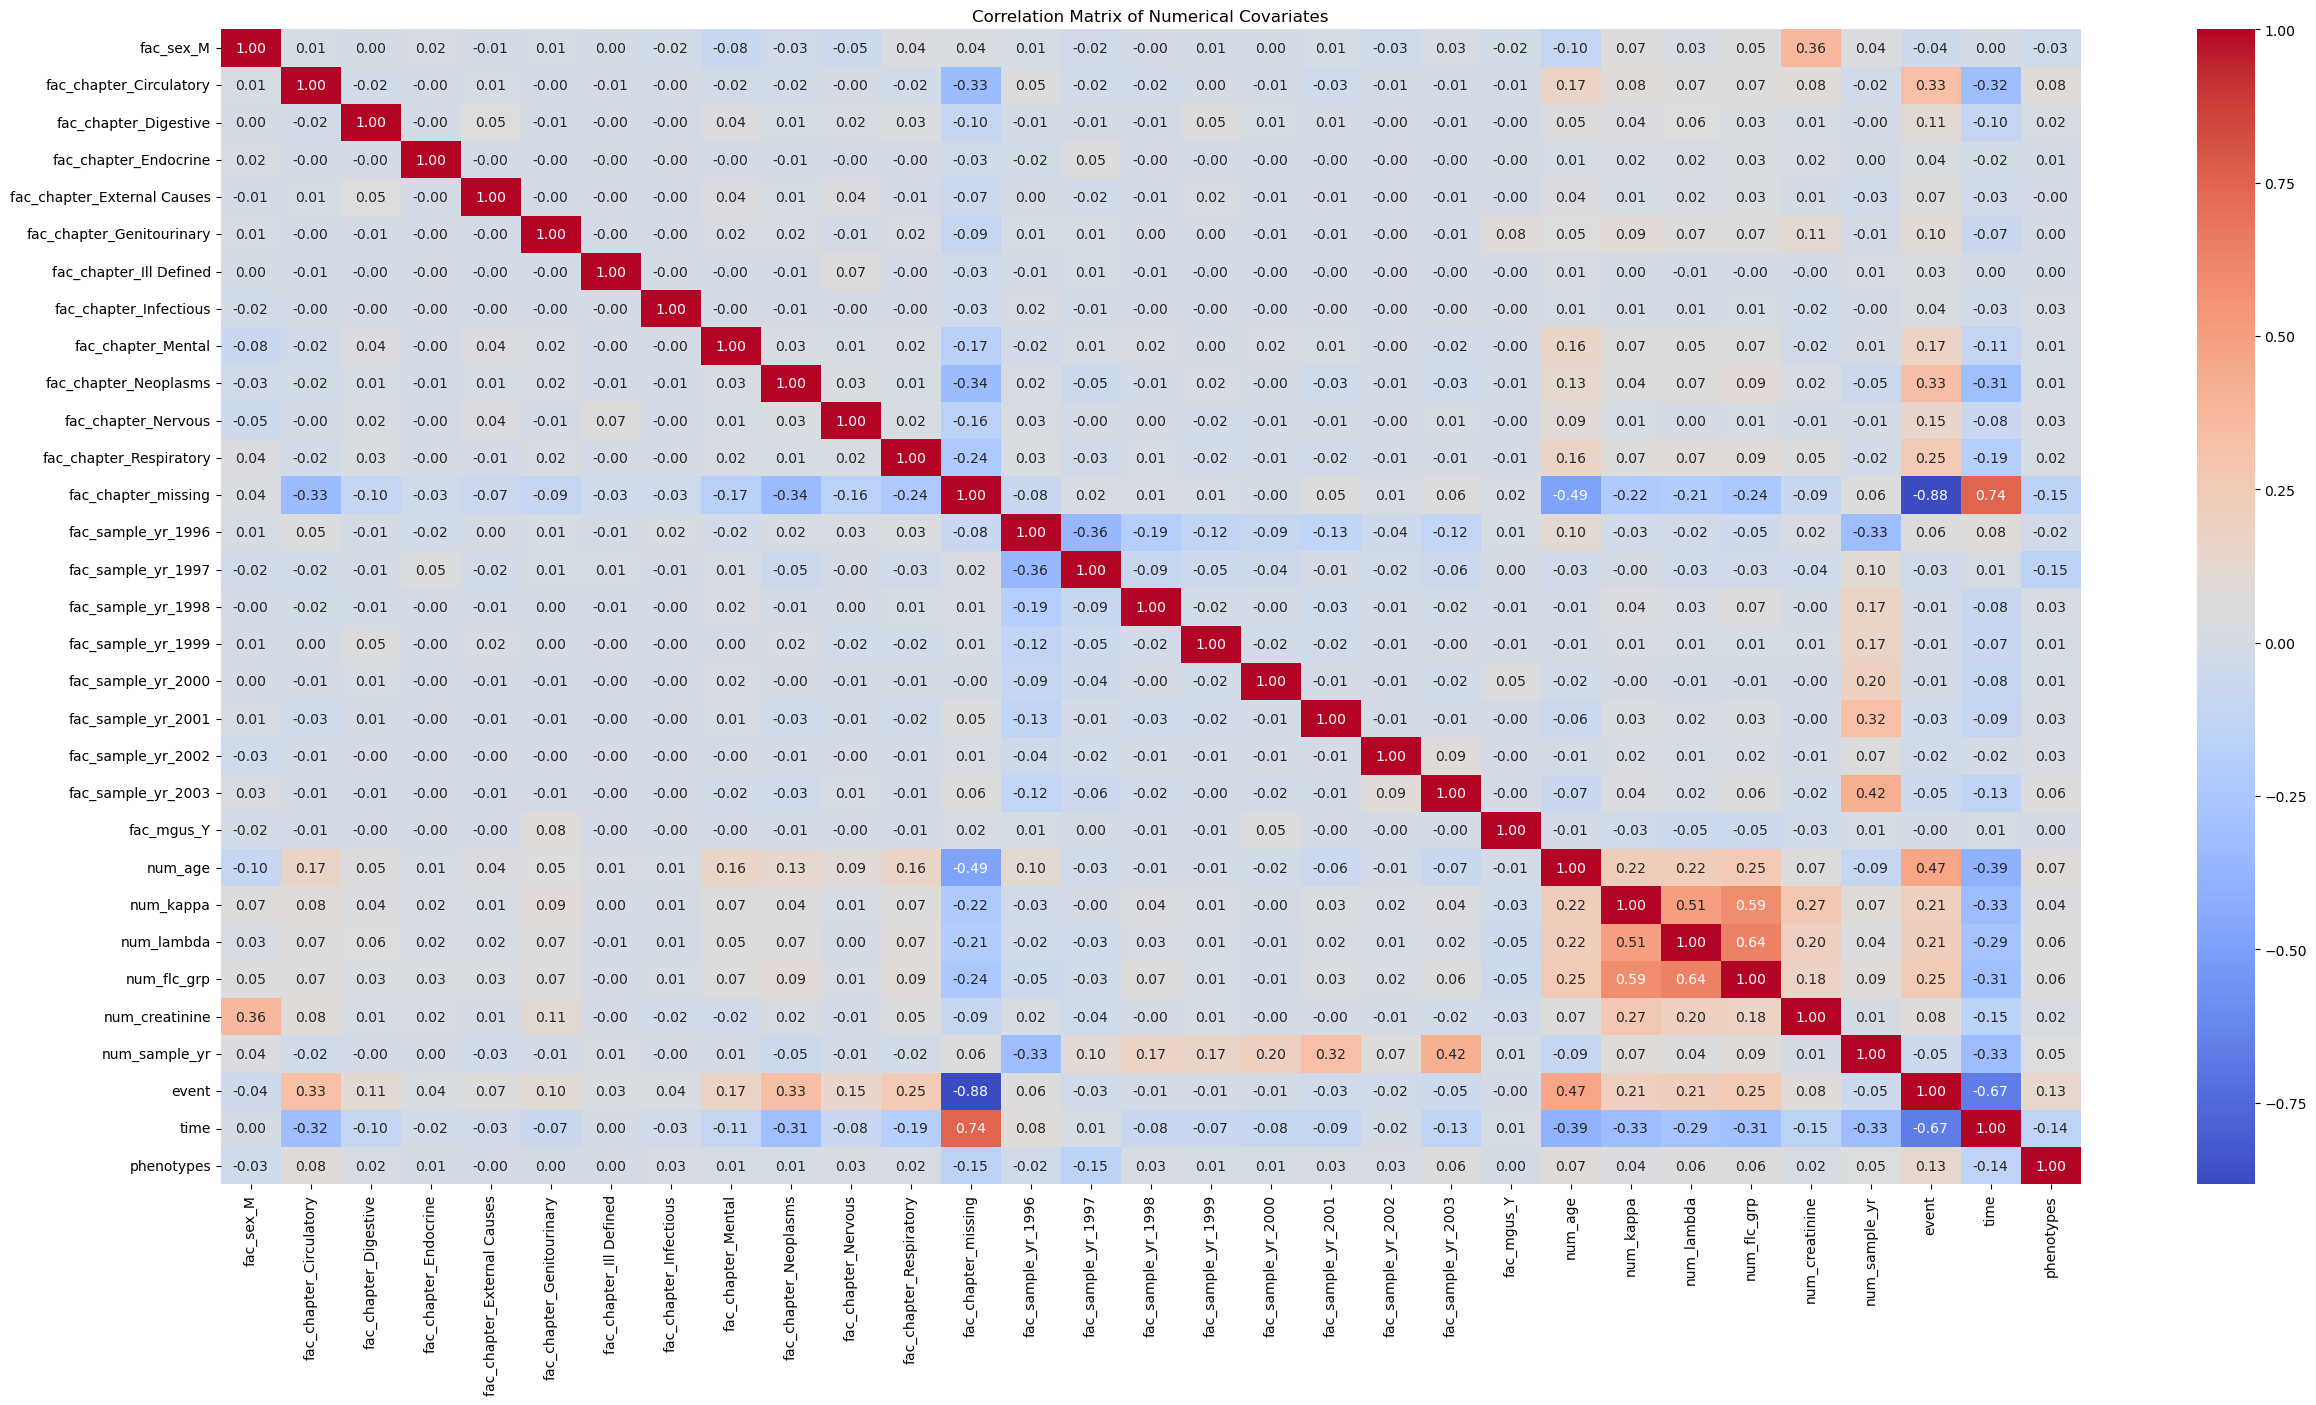
\includegraphics[scale=0.28]{Figures/EDA/corr.png}
    \caption{Correlation Matrix For Variables}
    \label{fig:corr_matrix}
\end{figure}
% \end{landscape}

\clearpage

\noindent The univariate analysis plots presented here offer a comprehensive view of the distribution of individual variables. While four one-hot encoded categorical features are shown for illustration of the non informative nature of these plots, the general tendency observed in the numerical variables is a roughly normal distribution centered around specific values. This suggests that the data is symmetrically distributed with most observations clustered around the mean, with some variation present across different numerical features.
\begin{figure}[h]
    \centering
    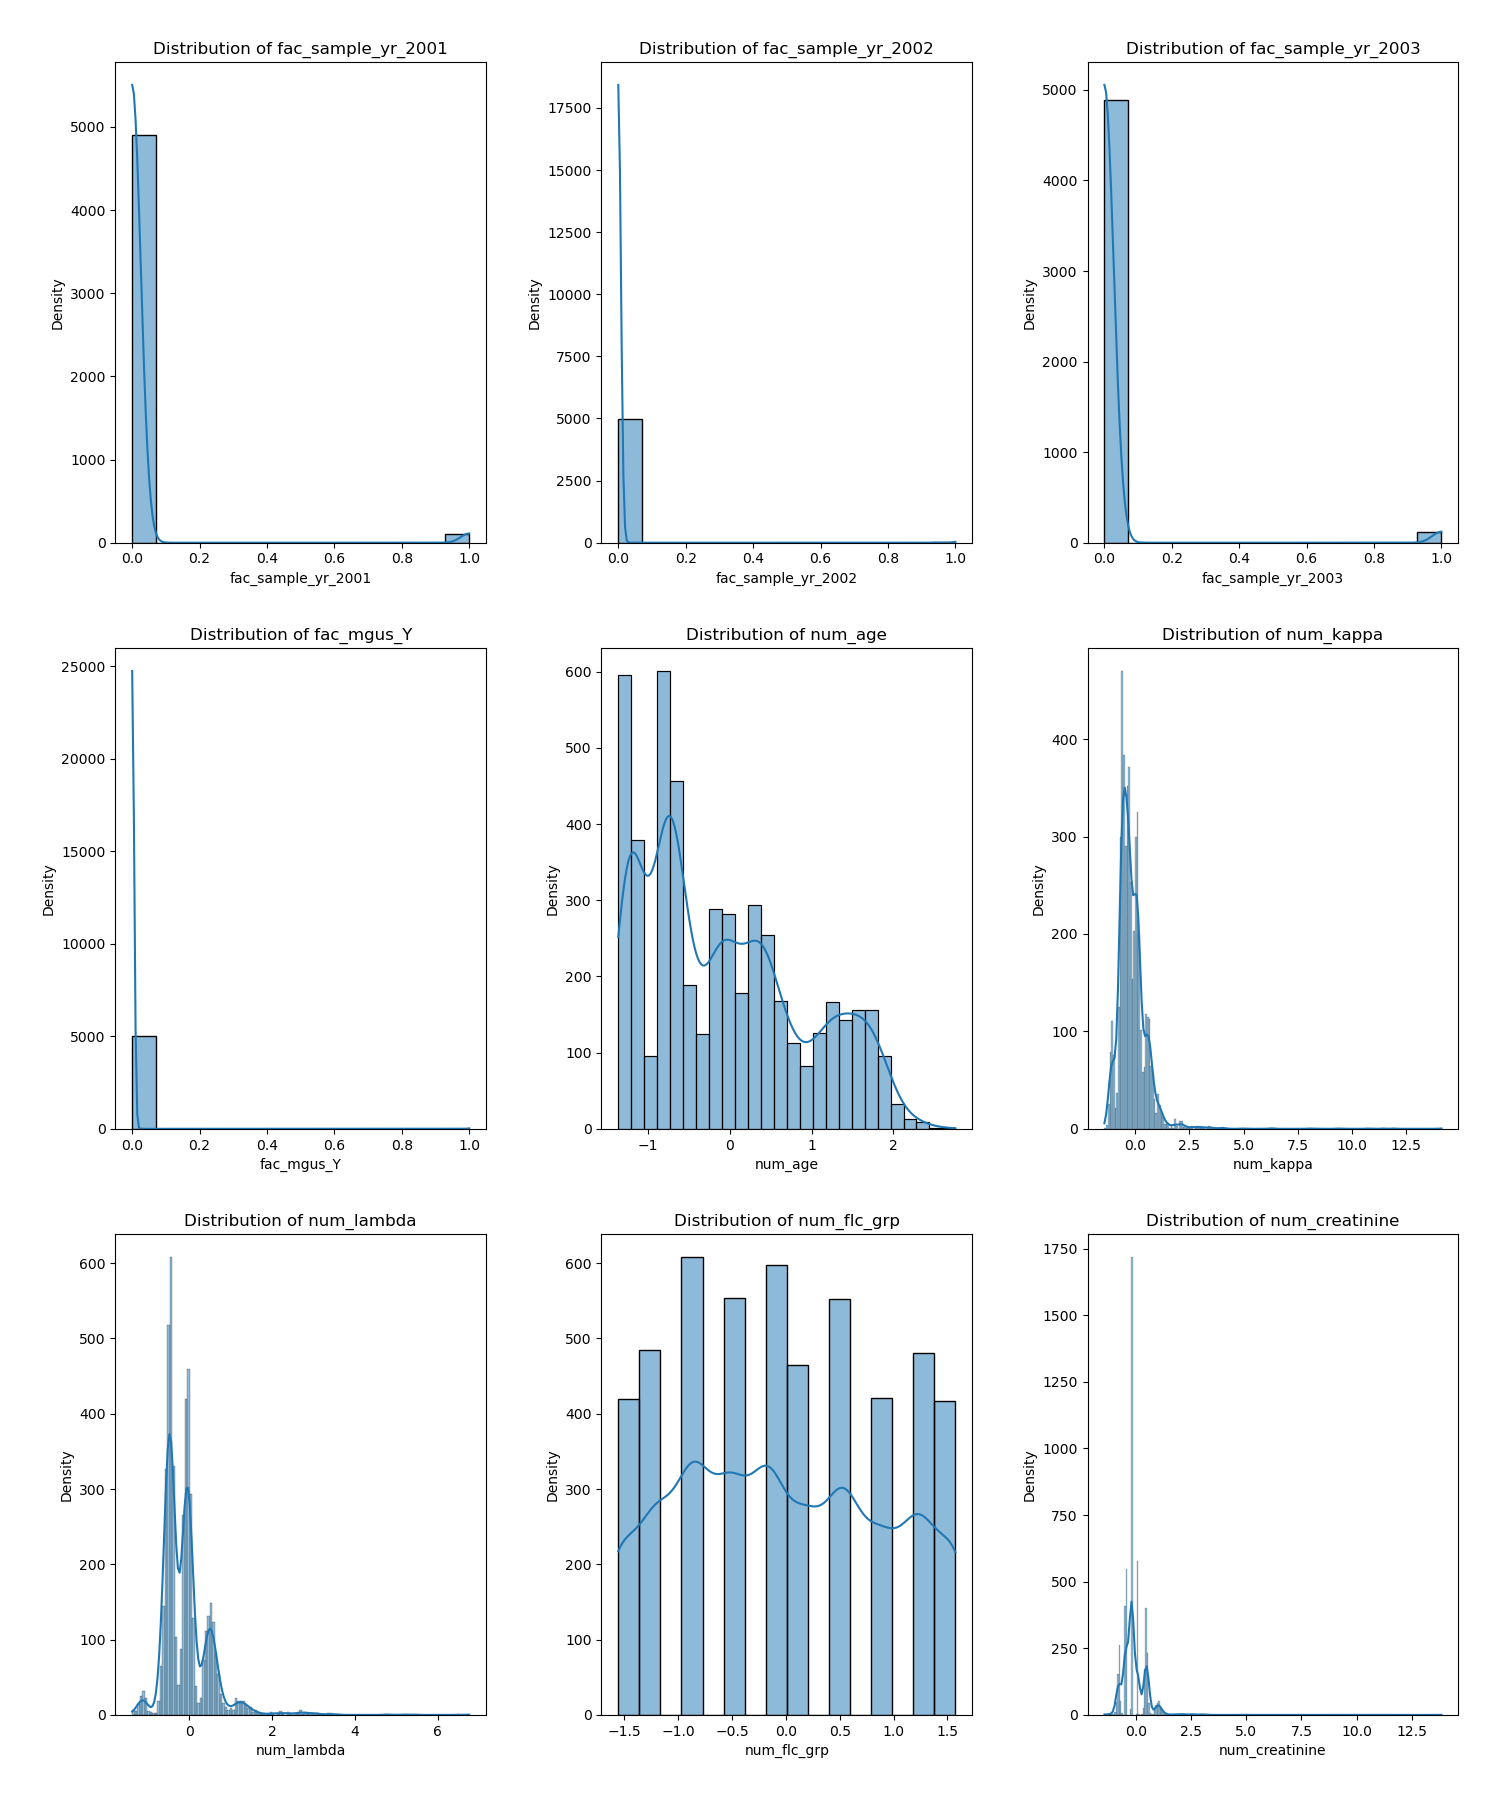
\includegraphics[scale=0.21]{Figures/EDA/uni3.png}
    \caption{Univariate Analysis Plots}
    \label{fig:uni1}
\end{figure}


\begin{figure}[h]
    \centering
    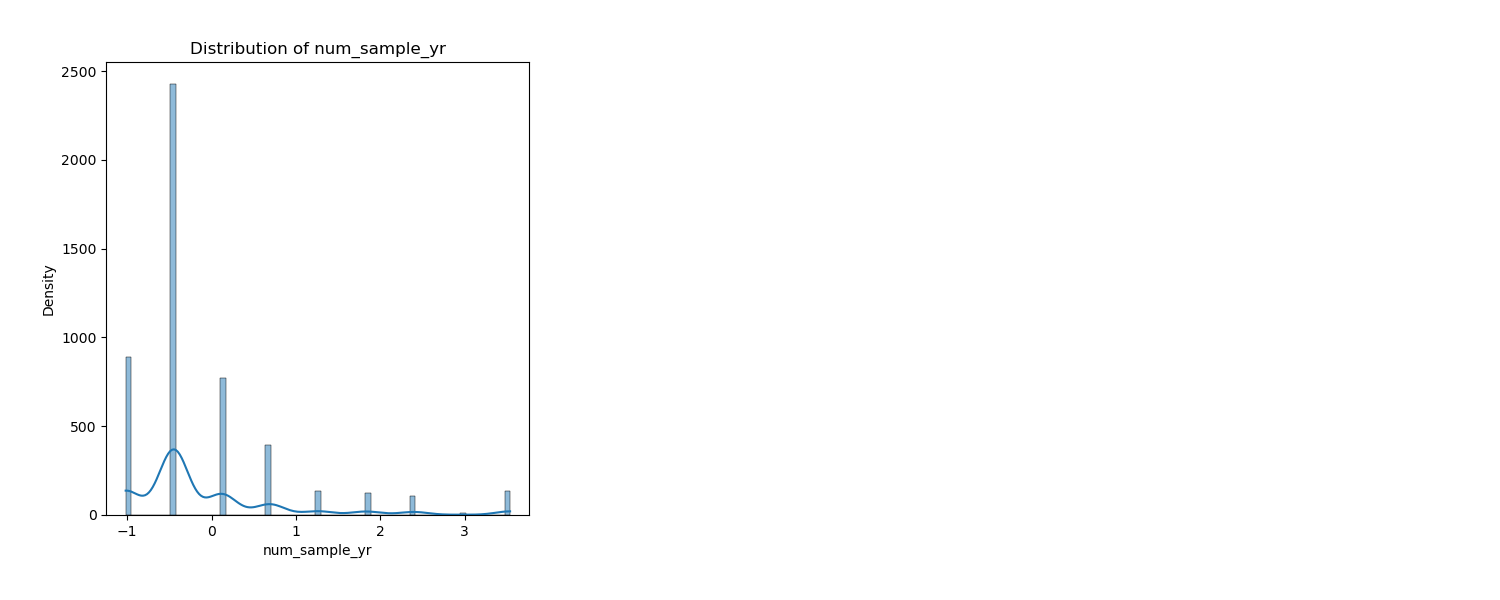
\includegraphics[scale=0.21]{Figures/EDA/uni4.png}
    \caption{Univariate Analysis Plots}
    \label{fig:uni2}
\end{figure}


\clearpage
\noindent These plots help visualize interactions, allowing us to explore possible correlations, trends, and dependencies. While most variables appear to follow a normal distribution, the age variable shows a noticeable skew, which is expected given that age naturally increases over time and influences other factors in the dataset. Understanding these patterns is crucial for developing robust predictive models and gaining deeper insights into the data.
\begin{figure}[h]
    \centering
    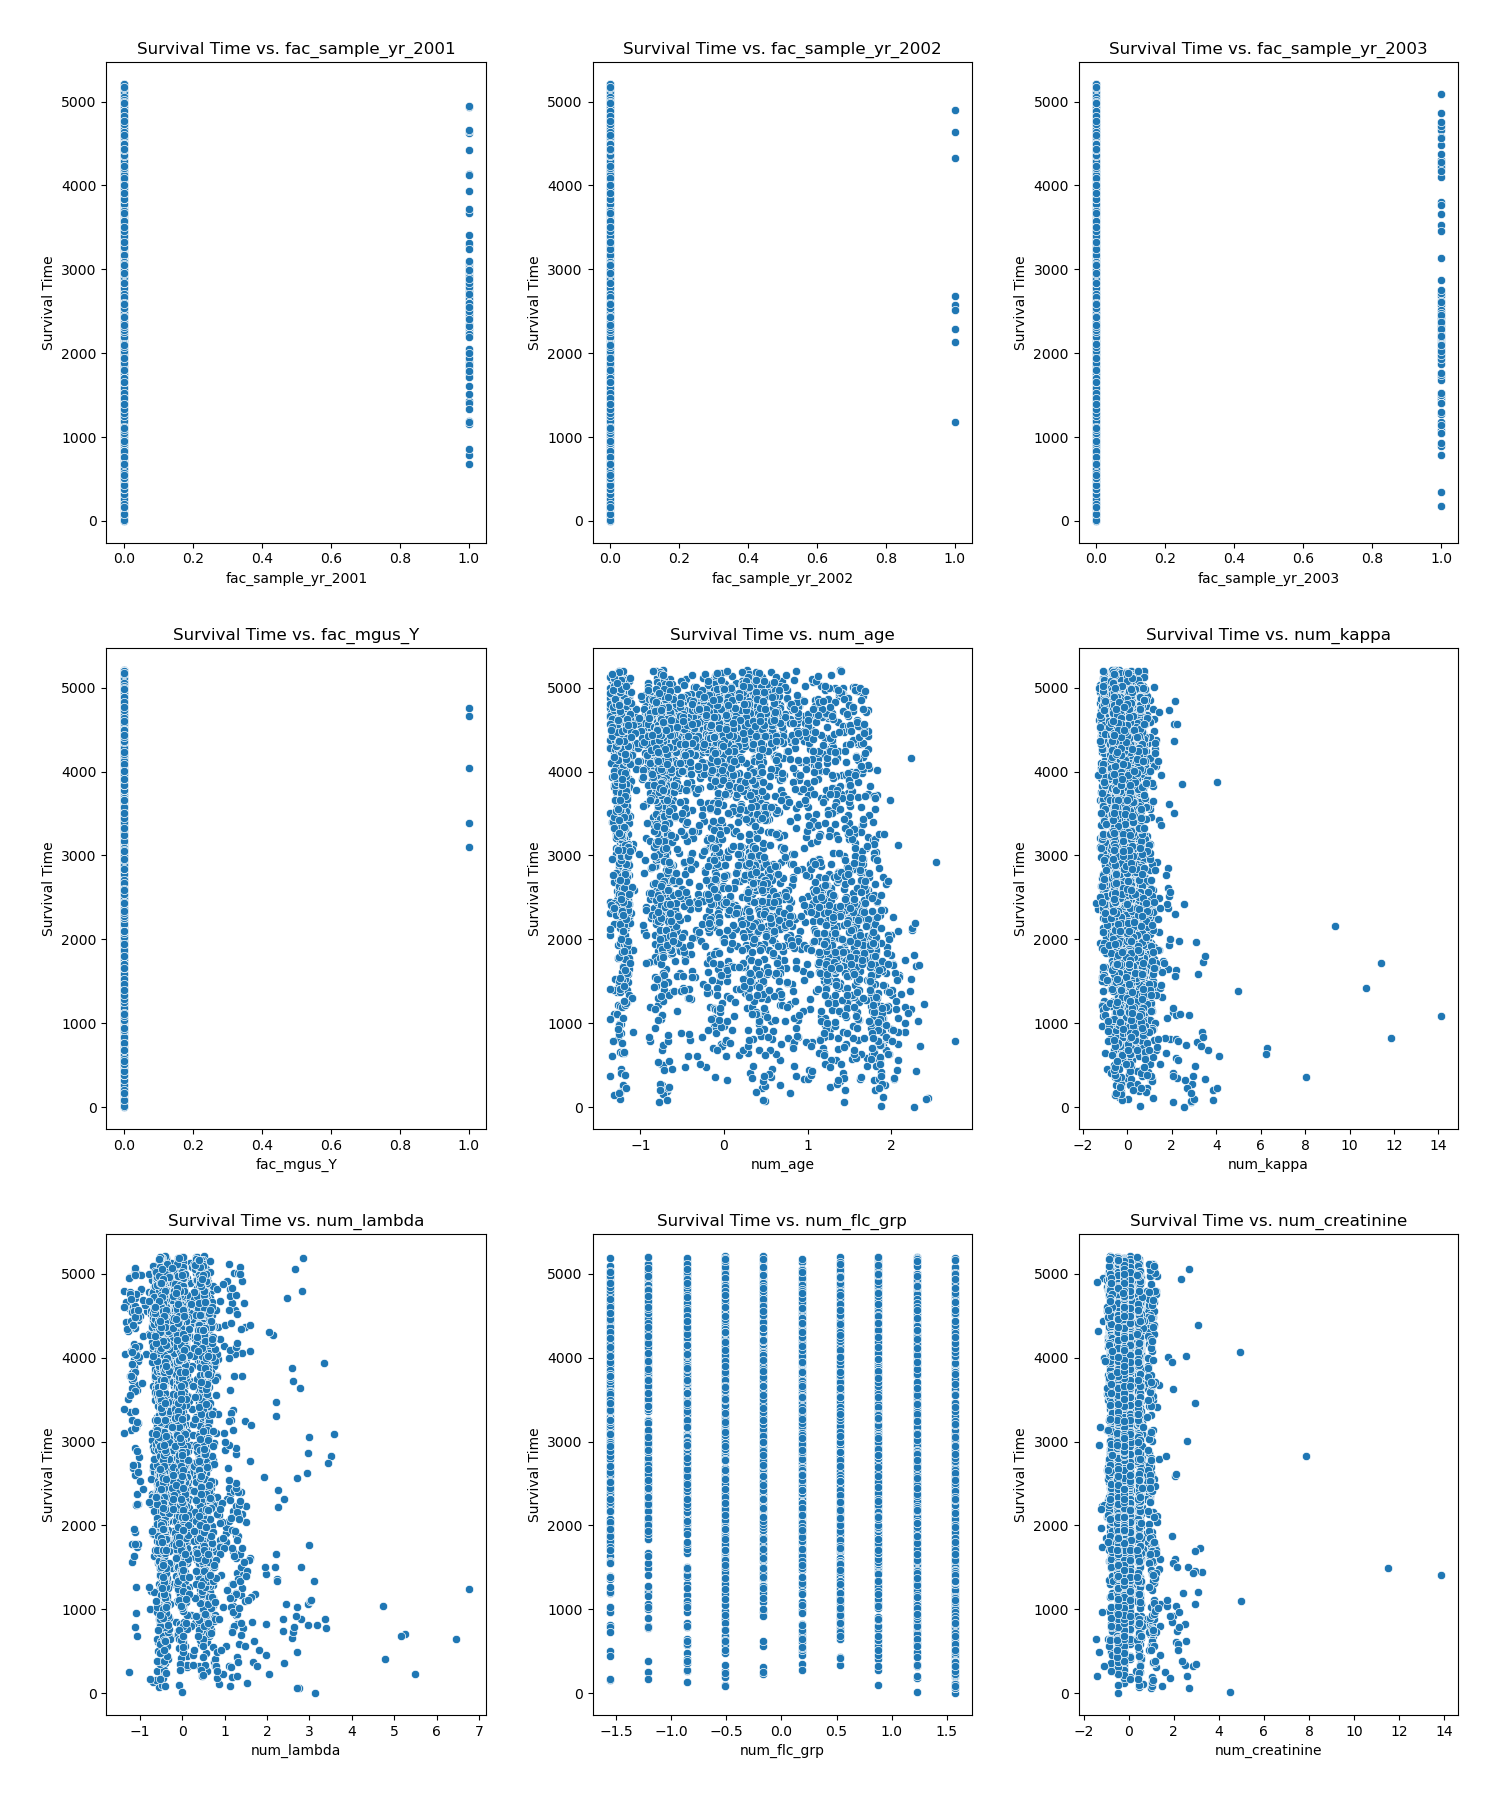
\includegraphics[scale=0.33]{Figures/EDA/scatter3.png}
    \caption{Bivariate Scatter Plots}
    \label{fig:scatter1}
\end{figure}

\begin{figure}[h]
    \centering
    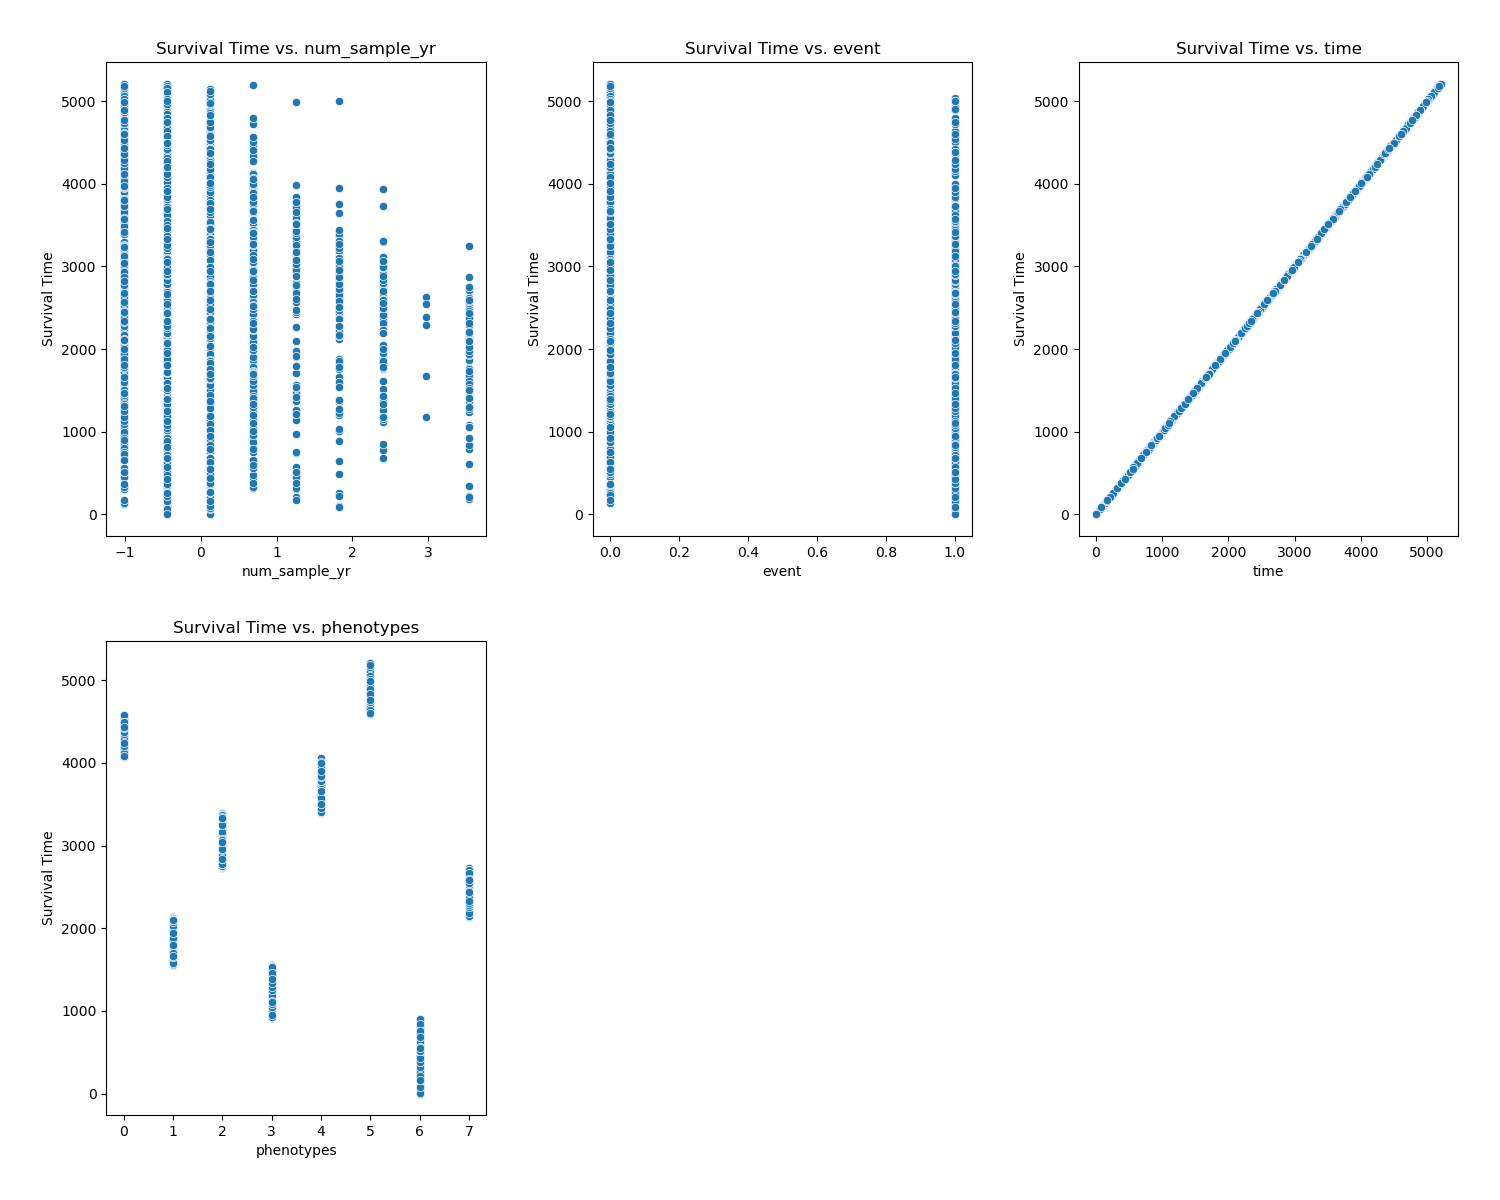
\includegraphics[scale=0.3]{Figures/EDA/scatter4.png}
    \caption{Bivariate Scatter Plots}
    \label{fig:scatter2}
\end{figure}

\begin{figure}[h]
    \centering
    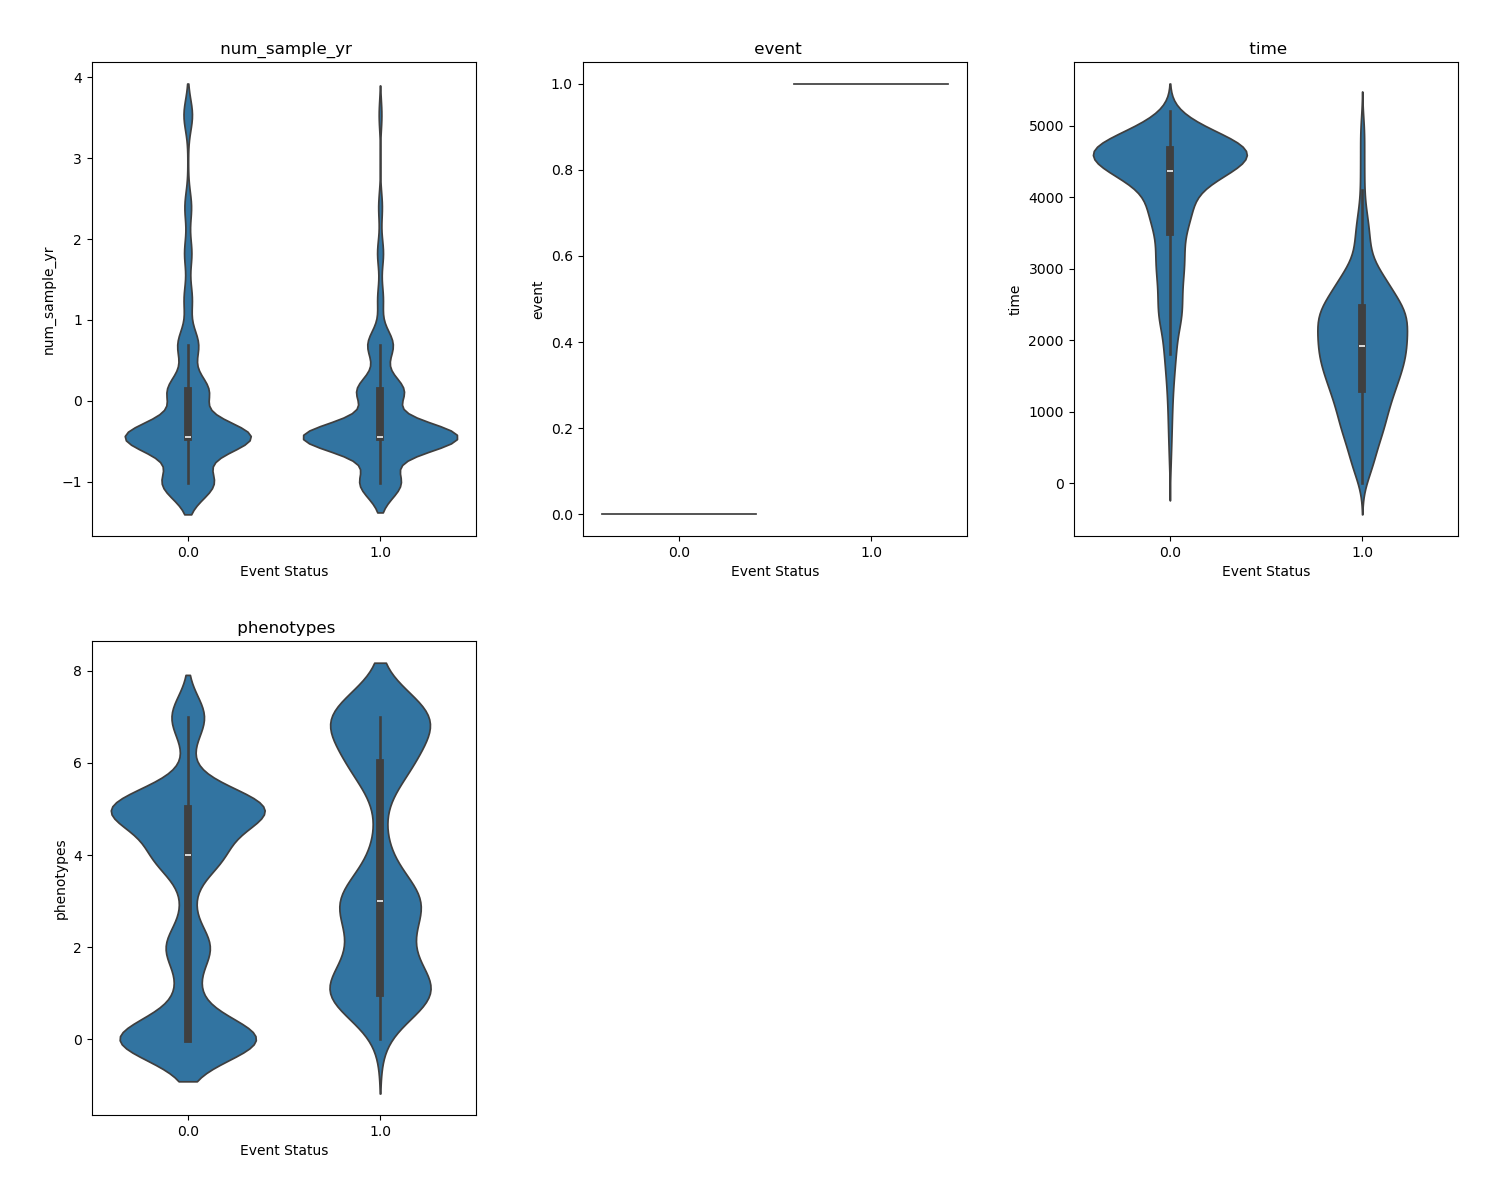
\includegraphics[scale=0.3]{Figures/EDA/violin4.png}
    \caption{Bivariate Violin Plots}
    \label{fig:your_label}
\end{figure}

\clearpage
\noindent The violin plots effectively highlight the detailed distribution of value ranges for each event type, revealing clear groupings across various features. A notable example is the num\_flc\_grp feature, where we observe a distinct pattern: positive values are predominantly associated with the occurrence of the event, while negative values are more common among patients who are still alive. This distinction provides valuable insight into how certain features influence the likelihood of survival or the occurrence of the event.
\begin{figure}[h]
    \centering
    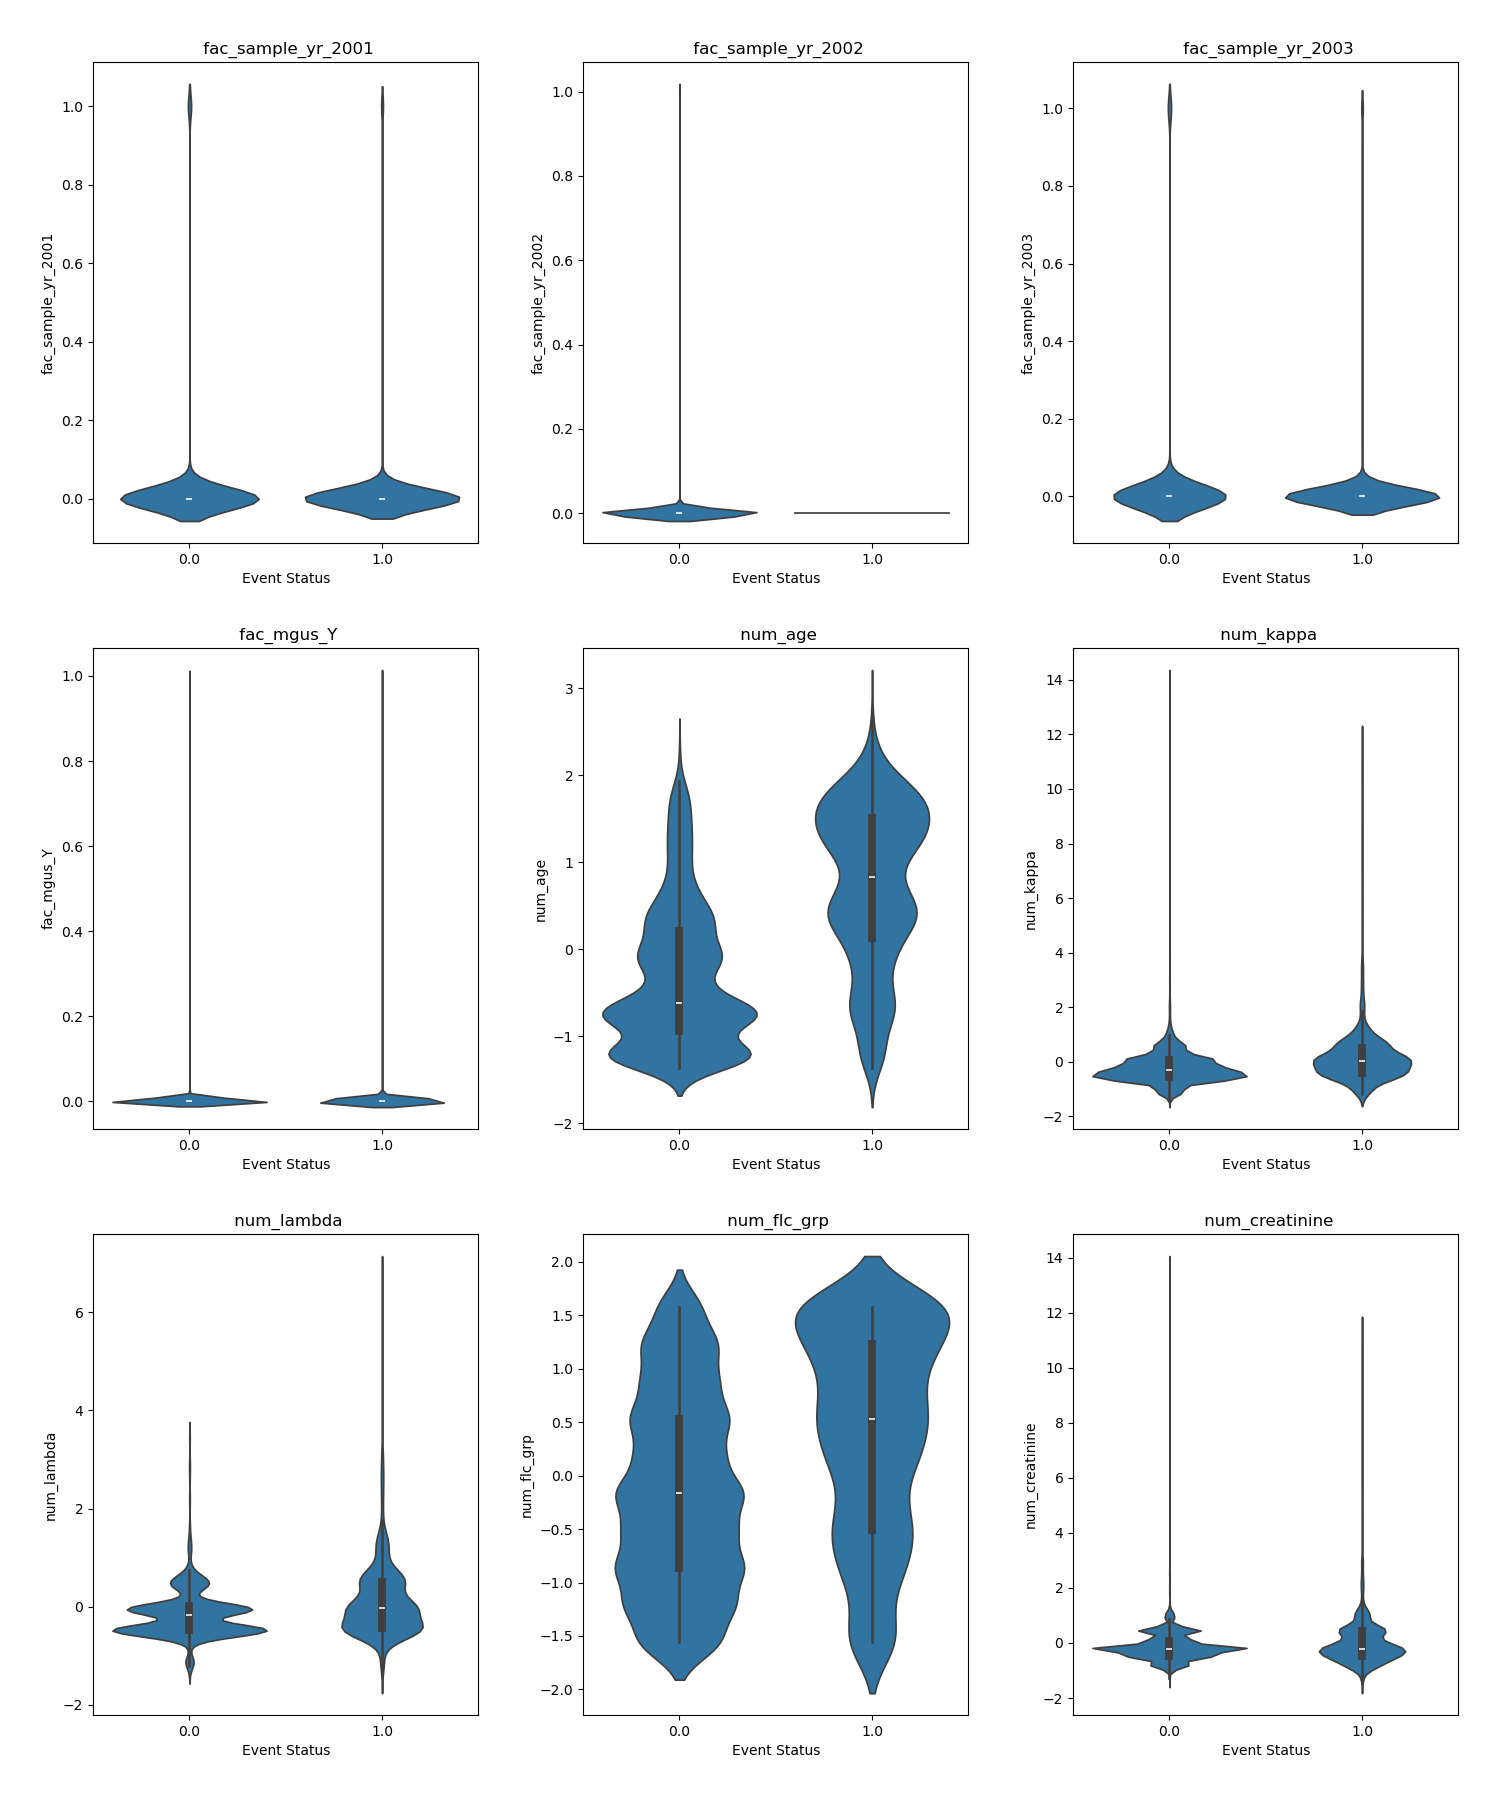
\includegraphics[scale=0.33]{Figures/EDA/violin3.png}
    \caption{Bivariate Violin Plots}
    \label{fig:your_label}
\end{figure}



\clearpage
\noindent  The per-variable censoring analysis, examines the distribution of censored observations across different variables. Censoring is a common occurrence in survival analysis, and this plot helps in understanding how censoring is distributed within the dataset. We can see the analysis will be preformed on a 75\% overall censoring distribution.
\begin{figure}[h]
    \centering
    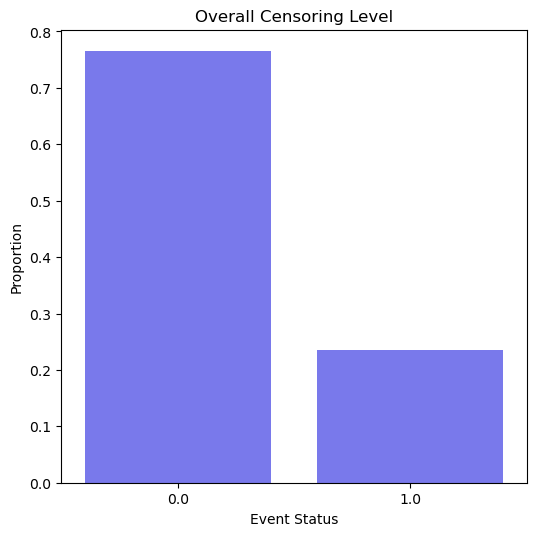
\includegraphics[scale=0.33]{Figures/EDA/censor_over.png}
    \caption{Per Variable Censoring}
    \label{fig:your_label}
\end{figure}

\begin{figure}[h]
    \centering
    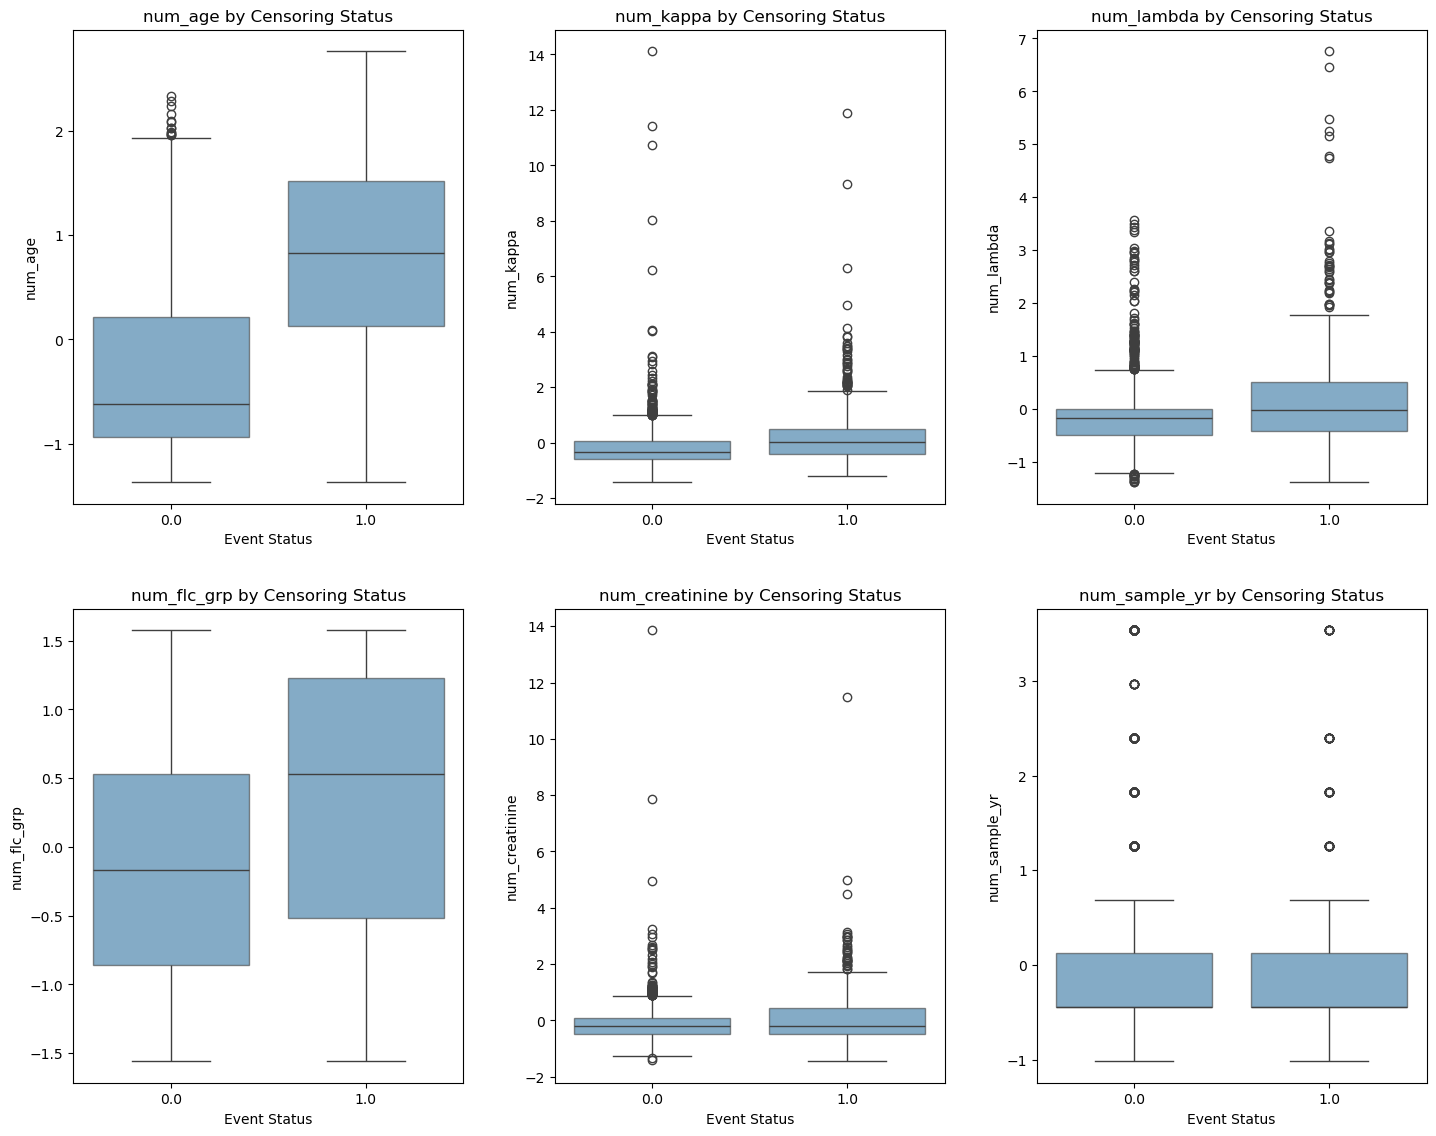
\includegraphics[scale=0.32]{Figures/EDA/censor.png}
    \caption{Numerical Censoring}
    \label{fig:your_label}
\end{figure}
\clearpage


\noindent In this figure, I present the results of the Auton-Survival phenotyping analysis, along with the compositions of the identified clusters. The phenotyping process involves grouping similar observations into clusters based on survival-related features. The figure highlights the characteristics of each cluster, offering insights into the heterogeneity within the population and helping to identify distinct survival patterns.
\begin{figure}[h]
    \centering
    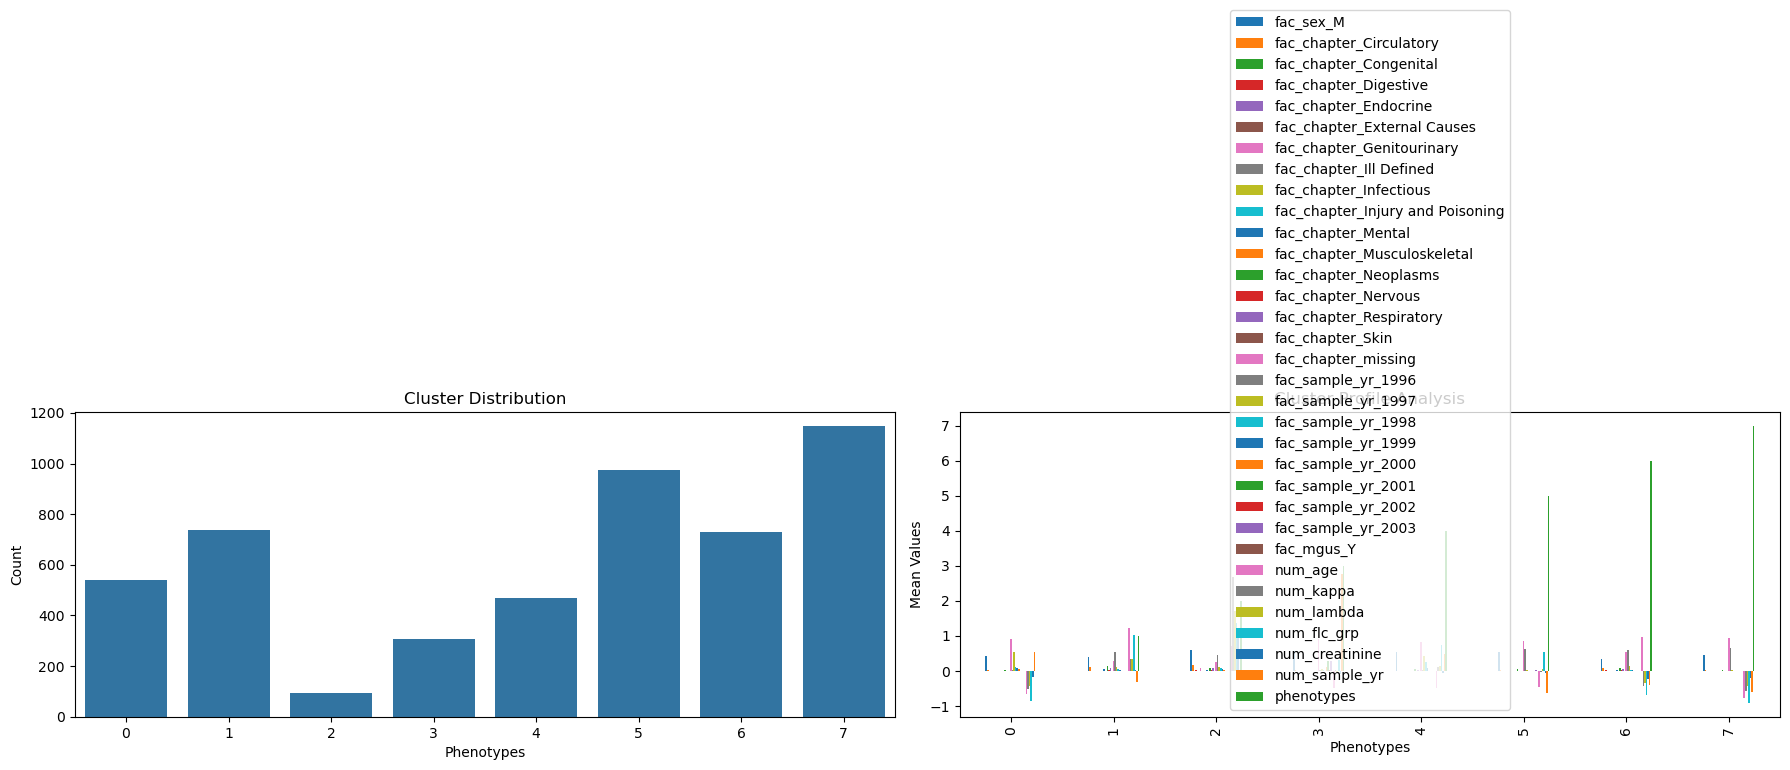
\includegraphics[scale=0.3]{Figures/EDA/clusters.png}
    \caption{Auton-Survival Phentotying Along with the cluster compositions}
    \label{fig:your_label}
\end{figure}
\clearpage
\noindent The Kaplan-Meier plot shown in this figure provides a survival analysis of the clusters identified in the phenotyping process. Each curve represents the survival probability over time for a specific cluster. This plot is useful for comparing the survival experiences of different groups within the dataset, revealing significant differences or similarities in survival rates across clusters.
\begin{figure}[h]
    \centering
    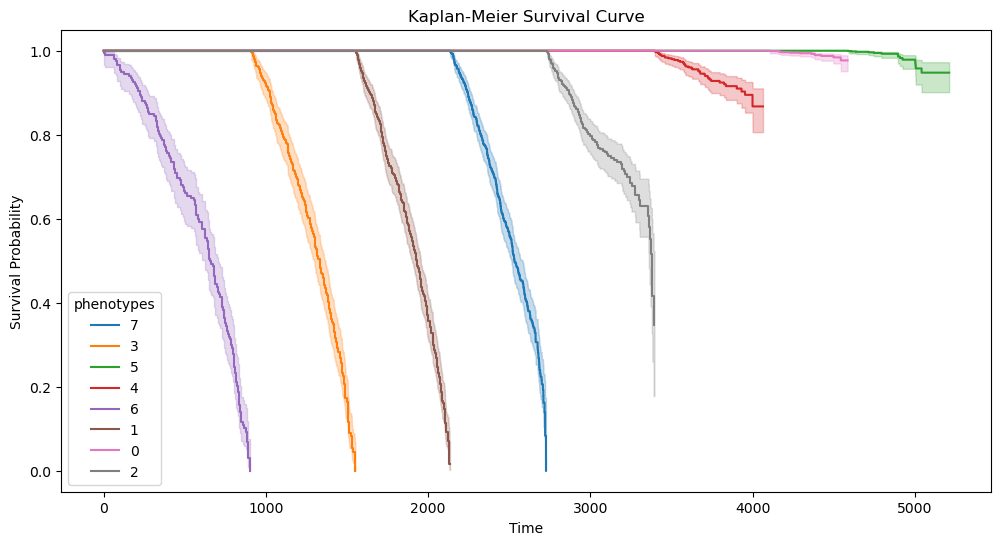
\includegraphics[scale=0.30]{Figures/EDA/cluster_kaplan.png}
    \caption{Kaplan-Meier Plot of the clusters}
    \label{fig:your_label}
\end{figure}

\noindent This figure illustrates the Neelson-Aalen cumulative hazard plot for the clusters identified in the phenotyping analysis. The plot displays the cumulative hazard function for each cluster, offering a different perspective on survival analysis compared to the Kaplan-Meier plot. It helps in understanding the risk accumulation over time and comparing the hazard rates across different clusters.
\begin{figure}[h]
    \centering
    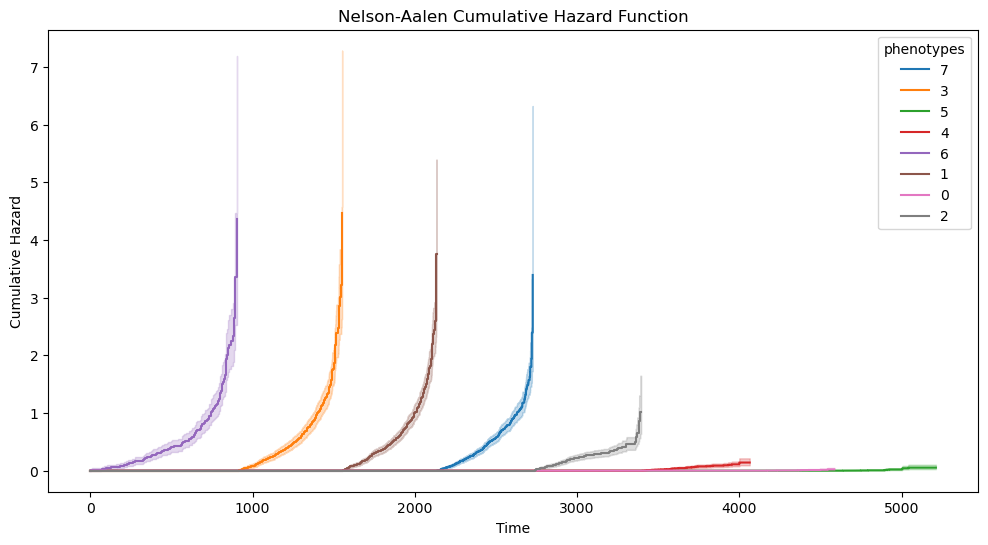
\includegraphics[scale=0.40]{Figures/EDA/cluster_neelson.png}
    \caption{Neelson-Aalen plot of the clusters}
    \label{fig:your_label}
\end{figure}


\section{Survival Analysis Case Study}
For the Case Study I present the results of running the models for just the Survival Variational Autoencoder generated data, I do this because the training of this model was faster by a factor of 10 times enabling generation after going back and changing data in the preporcessing stage as Issues arised during runtime of the models.

\subsection{Cox Proportional Hazards}
In the initial phase of the analysis, a Cox proportional hazards model was applied to the dataset. However, the model struggled with convergence, which was indicated by warning messages and issues related to matrix inversion and collinearity. These problems were addressed by following suggestions from the Lifeline documentation I talk about this in \ref{methods}. Specifically, I performed data thinning by dropping columns with low variance and potential complete separation. Additionally, I conducted a variance inflation factor (VIF) analysis to identify and remove highly collinear variables. These steps were crucial in stabilizing the model and resolving convergence issues.
\\\\
\noindent After applying the convergence checks and reprocessing the data, the Cox model successfully fit the dataset. The same preprocessed data was then reused for a Random Survival Forest (RSF) model to ensure consistency across the methods. Both models were evaluated on the test set, providing survival predictions, median survival estimates, and partial hazard calculations. The preprocessing steps proved effective in enabling the Cox model to converge and laid a solid foundation for comparison with the RSF model.

% \begin{figure}[h]
%     \centering
%     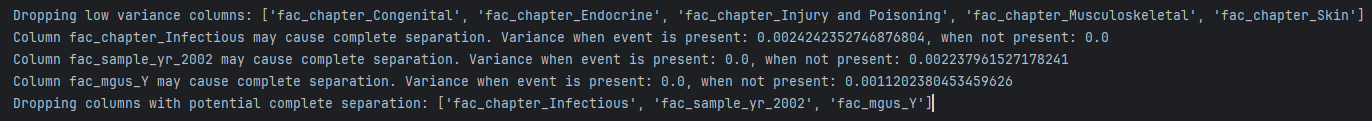
\includegraphics[width=\linewidth]{Figures/SURV/convergance_chaek.png}
%     \caption{Convergance Output}
%     \label{fig:conv_out}
% \end{figure}


\begin{figure}[h]
    \centering
    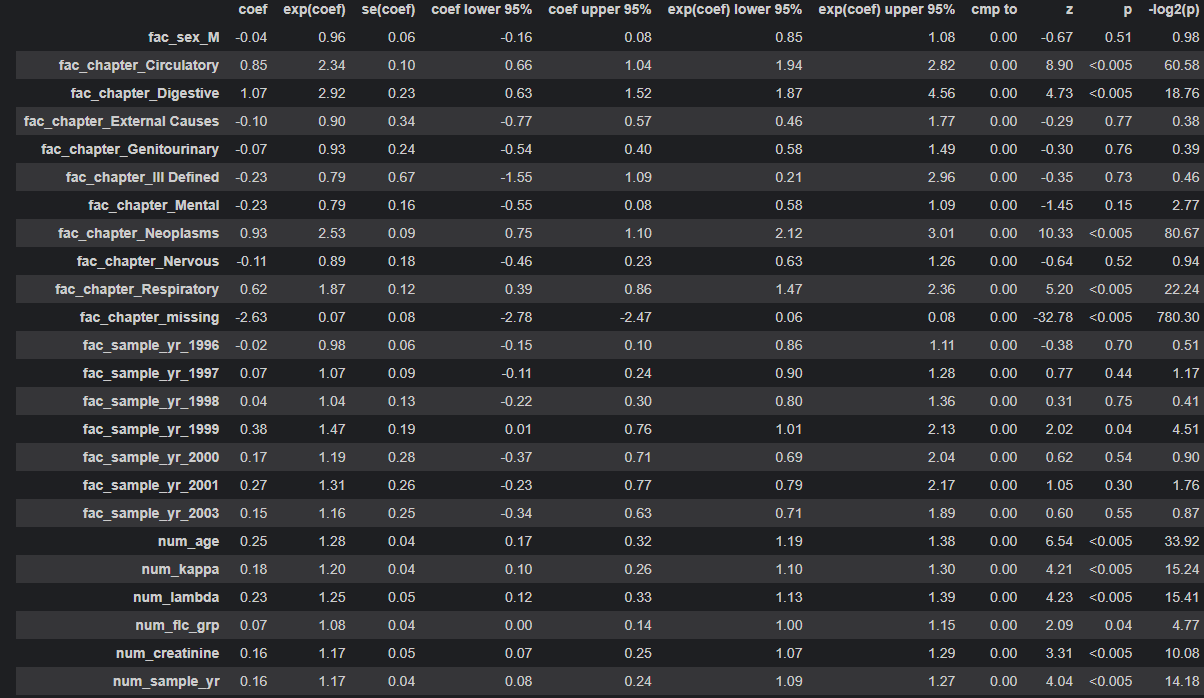
\includegraphics[width=\linewidth]{Figures/SURV/covariates.png}
    \caption{coefficient values}
    \label{fig:your_label}
\end{figure}

\begin{figure}[h]
    \centering
    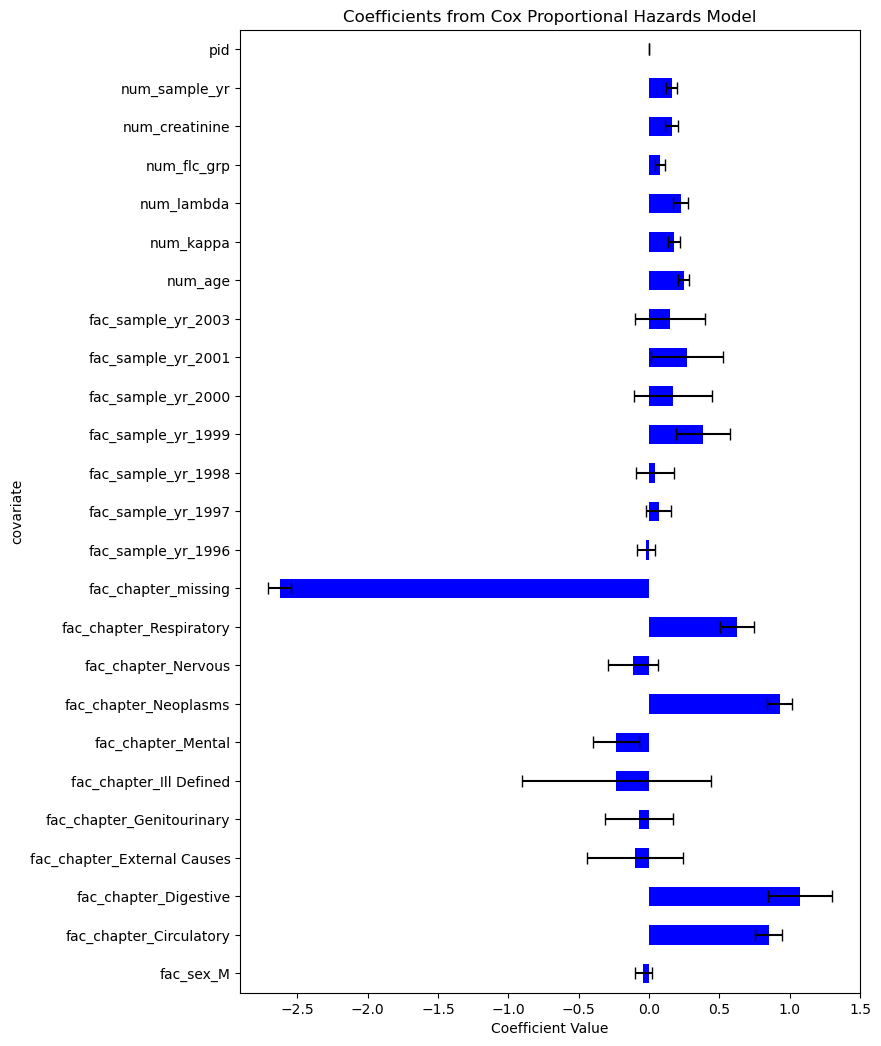
\includegraphics[width=\linewidth]{Figures/SURV/cox_cov.png}
    \caption{Boxplots of coefficients}
    \label{fig:your_label}
\end{figure}

\begin{figure}[h]
    \centering
    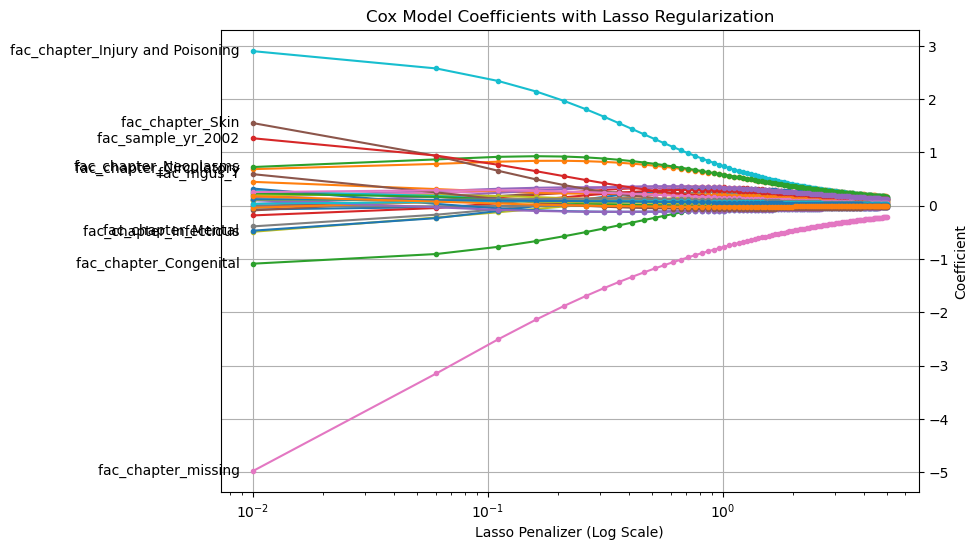
\includegraphics[width=\linewidth]{Figures/SURV/lasso_reg.png}
    \caption{Lasso regularized coefficient panning closer to zero}
    \label{fig:your_label}
\end{figure}

\begin{figure}[h]
    \centering
    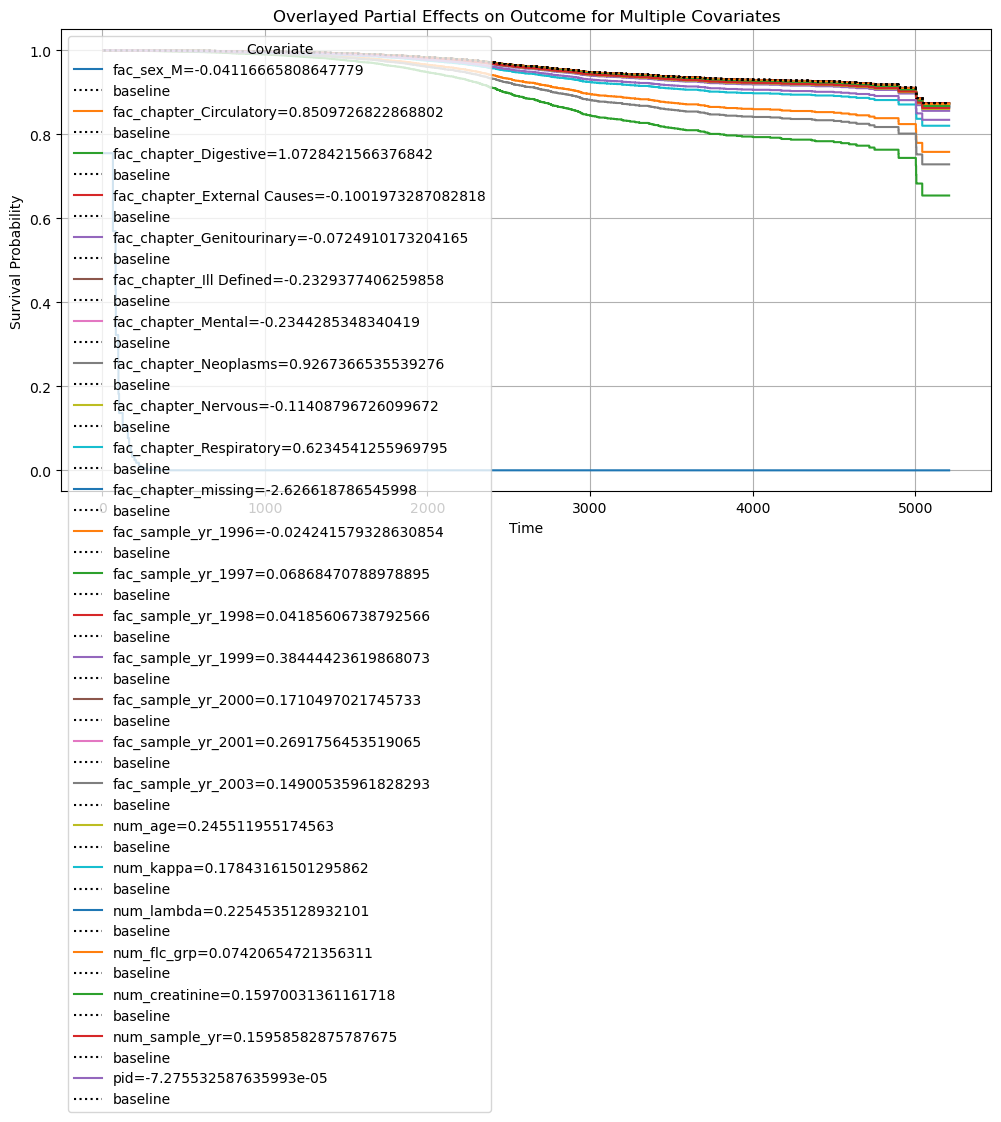
\includegraphics[width=\linewidth]{Figures/SURV/cox_overlay.png}
    \caption{Survival curves for covariates}
    \label{fig:your_label}
\end{figure}


\begin{figure}[h]
    \centering
    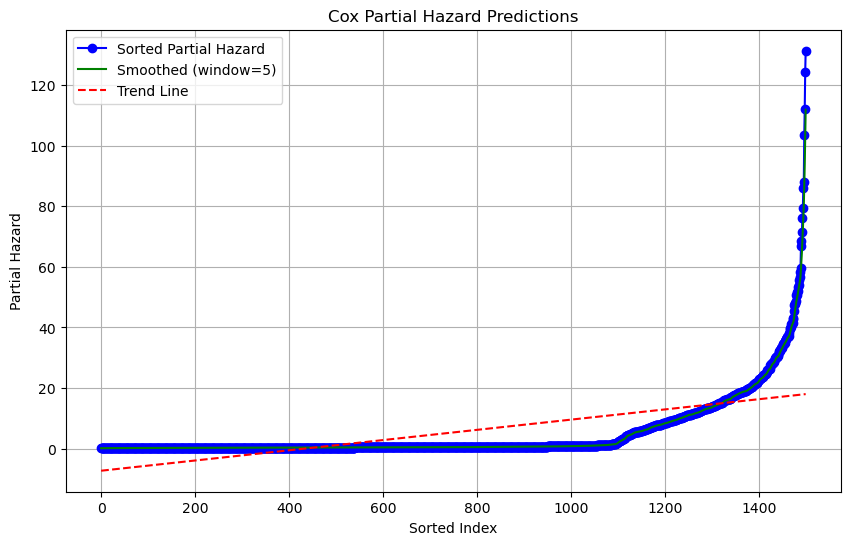
\includegraphics[width=\linewidth]{Figures/SURV/cox_hazard.png}
    \caption{Mean Hazard Visualisation}
    \label{fig:your_label}
\end{figure}

\clearpage
\subsubsection*{Assumption Check}
\begin{table}[H]
    \centering
    \caption{Test Statistics, p-values, and -log2(p) for Different Variables}
    \tiny
    \begin{tabular}{|l|l|c|c|c|}
    \hline
    \textbf{Variable}                & \textbf{Test Type} & \textbf{Test Statistic} & \textbf{p-value} & \textbf{-log2(p)} \\ \hline
    fac\_chapter\_Circulatory        & km   & 16.29 & <0.005 & 14.16 \\ \hline
                                    & rank & 17.65 & <0.005 & 15.20 \\ \hline
    fac\_chapter\_Digestive          & km   & 0.97  & 0.32   & 1.63  \\ \hline
                                    & rank & 0.95  & 0.33   & 1.60  \\ \hline
    fac\_chapter\_External Causes    & km   & 2.86  & 0.09   & 3.46  \\ \hline
                                    & rank & 2.24  & 0.13   & 2.90  \\ \hline
    fac\_chapter\_Genitourinary      & km   & 0.03  & 0.87   & 0.20  \\ \hline
                                    & rank & 0.03  & 0.86   & 0.22  \\ \hline
    fac\_chapter\_Ill Defined        & km   & 0.00  & 0.95   & 0.07  \\ \hline
                                    & rank & 0.00  & 0.95   & 0.07  \\ \hline
    fac\_chapter\_Mental             & km   & 0.41  & 0.52   & 0.93  \\ \hline
                                    & rank & 0.32  & 0.57   & 0.80  \\ \hline
    fac\_chapter\_Neoplasms          & km   & 5.65  & 0.02   & 5.84  \\ \hline
                                    & rank & 5.82  & 0.02   & 5.98  \\ \hline
    fac\_chapter\_Nervous            & km   & 1.00  & 0.32   & 1.65  \\ \hline
                                    & rank & 0.90  & 0.34   & 1.54  \\ \hline
    fac\_chapter\_Respiratory        & km   & 0.72  & 0.40   & 1.34  \\ \hline
                                    & rank & 0.90  & 0.34   & 1.54  \\ \hline
    fac\_chapter\_missing            & km   & 57.74 & <0.005 & 44.93 \\ \hline
                                    & rank & 58.70 & <0.005 & 45.63 \\ \hline
    fac\_sample\_yr\_1996            & km   & 1.04  & 0.31   & 1.70  \\ \hline
                                    & rank & 1.00  & 0.32   & 1.65  \\ \hline
    fac\_sample\_yr\_1997            & km   & 0.34  & 0.56   & 0.84  \\ \hline
                                    & rank & 0.37  & 0.54   & 0.88  \\ \hline
    fac\_sample\_yr\_1998            & km   & 0.04  & 0.85   & 0.23  \\ \hline
                                    & rank & 0.01  & 0.91   & 0.13  \\ \hline
    fac\_sample\_yr\_1999            & km   & 0.89  & 0.34   & 1.54  \\ \hline
                                    & rank & 0.96  & 0.33   & 1.61  \\ \hline
    fac\_sample\_yr\_2000            & km   & 0.49  & 0.48   & 1.05  \\ \hline
                                    & rank & 0.58  & 0.45   & 1.16  \\ \hline
    fac\_sample\_yr\_2001            & km   & 0.11  & 0.73   & 0.44  \\ \hline
                                    & rank & 0.12  & 0.73   & 0.45  \\ \hline
    fac\_sample\_yr\_2003            & km   & 0.23  & 0.63   & 0.67  \\ \hline
                                    & rank & 0.25  & 0.62   & 0.70  \\ \hline
    fac\_sex\_M                      & km   & 0.45  & 0.50   & 0.99  \\ \hline
                                    & rank & 0.36  & 0.55   & 0.86  \\ \hline
    num\_age                         & km   & 1.34  & 0.25   & 2.01  \\ \hline
                                    & rank & 1.32  & 0.25   & 2.00  \\ \hline
    num\_creatinine                  & km   & 5.45  & 0.02   & 5.68  \\ \hline
                                    & rank & 5.59  & 0.02   & 5.79  \\ \hline
    num\_flc\_grp                    & km   & 0.06  & 0.80   & 0.32  \\ \hline
                                    & rank & 0.06  & 0.81   & 0.31  \\ \hline
    num\_kappa                       & km   & 0.13  & 0.72   & 0.47  \\ \hline
                                    & rank & 0.12  & 0.73   & 0.46  \\ \hline
    num\_lambda                      & km   & 0.13  & 0.72   & 0.48  \\ \hline
                                    & rank & 0.08  & 0.77   & 0.37  \\ \hline
    num\_sample\_yr                  & km   & 1.29  & 0.26   & 1.96  \\ \hline
                                    & rank & 1.39  & 0.24   & 2.07  \\ \hline
    \end{tabular}
    \end{table}

\noindent The variable \texttt{num\_creatinine} failed the non-proportional hazards test, as indicated by the p-value of 0.0181, is likely due to a violation of the proportional hazards assumption. This assumption requires that the effect of the covariate on the hazard function remains constant over time \parencite{kalbfleisch_fifty_2023}. When a variable fails this test, it suggests that its relationship with the hazard may change over time, which could be due to several factors:

\begin{figure}[h]
    \centering
    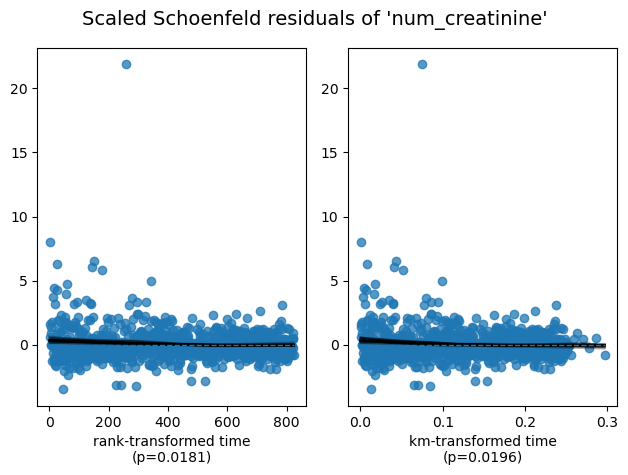
\includegraphics[width=\linewidth]{Figures/SURV/schoen1.png}
    \caption{Schoenfeld Residuals for num\_creatinine}
    \label{fig:your_label}
\end{figure}

\begin{itemize}
    \item \textbf{Incorrect Functional Form:} The relationship between \texttt{num\_creatinine} and the outcome might not be linear, and missing non-linear terms could be causing the violation \parencite{harrell__regression_2015}. The proportional hazards test is highly sensitive to such misspecifications.
    \item \textbf{Non-Linearity:} The variable \texttt{num\_creatinine} may have different effects at different levels, which could be addressed by transforming the variable or using binning (e.g., with \texttt{pd.cut}) to categorize it. This approach helps account for non-proportional effects by stratifying the data.
    \item \textbf{Time-Varying Effects:} The effect of \texttt{num\_creatinine} on the hazard may change over time, suggesting that adding an interaction term with time could better capture this dynamic relationship.
\end{itemize}

\noindent \texttt{num\_creatinine} may not meet the proportional hazards assumption due to non-linearity or time-varying effects, but can be addressed by modifying the functional form, using stratification, or introducing interaction terms with time.



\clearpage




\subsection{Random Survival Forest}

In the initial Random Survival Forest (RSF) model, a static set of parameters was used, producing expected results. However, to improve performance, I introduced dynamic parameter tuning, similar to the approach used in Lasso models with varying alpha parameters. This involved using GridSearchCV with a search grid of 12 parameters, allowing the model to explore various configurations to find the optimal combination.
\\\\
\noindent While this dynamic tuning enhanced the model's accuracy, it significantly increased training time, with each run taking an average of one hour. Despite the longer processing time, the parameter-tuned RSF model provided better results, with improved survival function predictions and more accurate cumulative hazard estimates. The grid search also helped to identify important features through permutation importance analysis, offering deeper insights into the model's performance.
\begin{figure}[h]
    \centering
    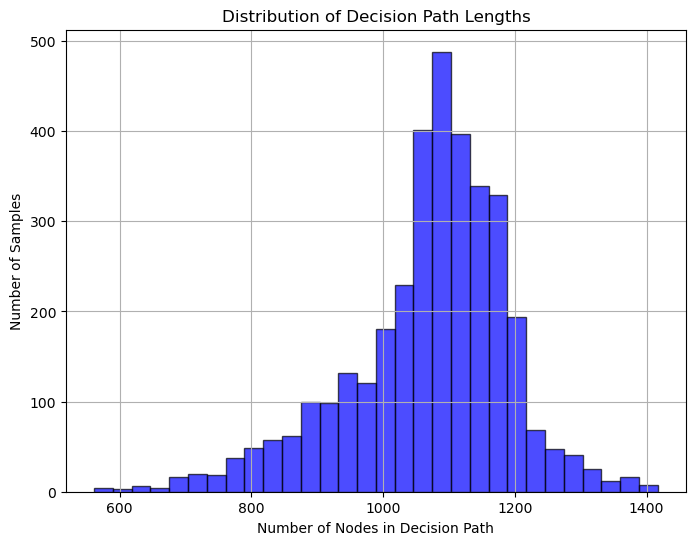
\includegraphics[scale=0.6]{Figures/SURV/rsf_paths.png}
    \caption{Descision Tree Matrix Visualisation}
    \label{fig:des_path}
\end{figure}

\clearpage
\begin{figure}[h]
    \centering
    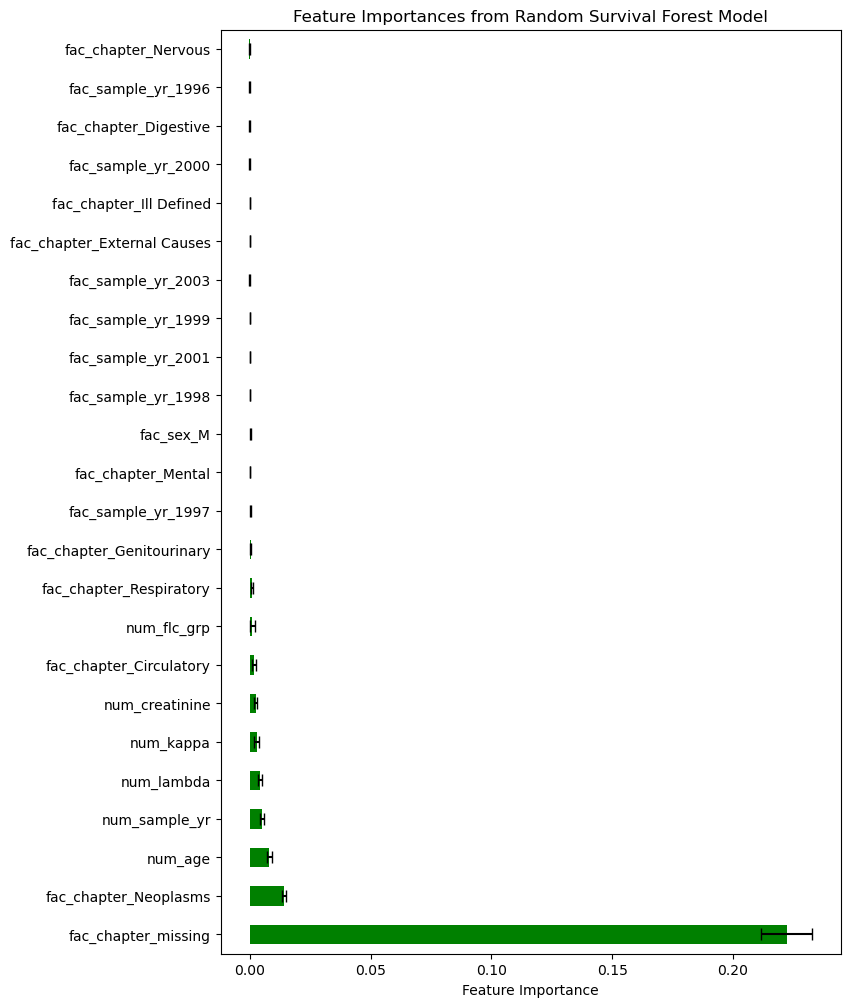
\includegraphics[width=\linewidth]{Figures/SURV/rsf_imp.png}
    \caption{Variable Importance Boxplots}
    \label{fig:var_imp}
\end{figure}



\clearpage

\begin{figure}[h]
    \centering
    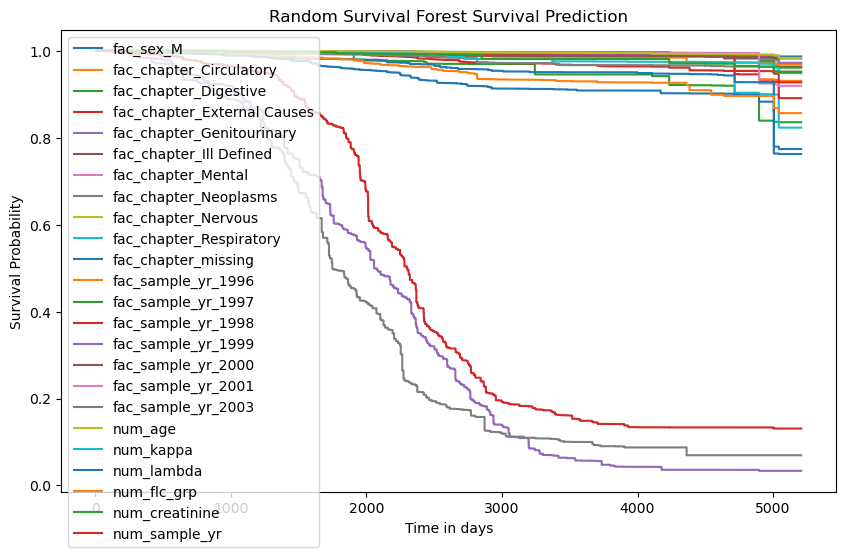
\includegraphics[scale=0.50]{Figures/SURV/rsf_survival.png}
    \caption{RSF Surival Curves}
    \label{fig:rsf_surv}
\end{figure}

\begin{figure}[h]
    \centering
    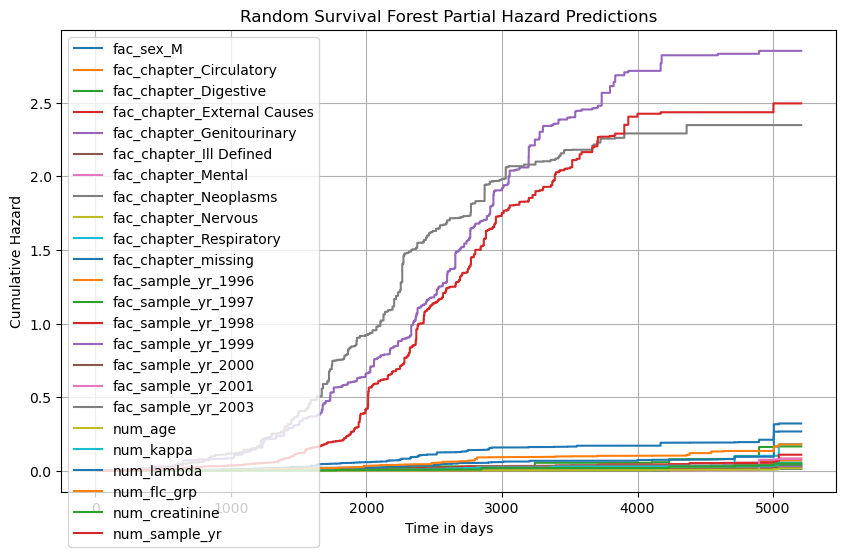
\includegraphics[scale=0.50]{Figures/SURV/rsf_hazard.png}
    \caption{RSF Hazard Curves}
    \label{fig:rsf_haz}
\end{figure}

\clearpage
\subsection{Models comparison} 

The final metrics as described in \ref{design} is shown here:

\begin{table}[h!]
    \centering
    \begin{tabular}{|l|l|l|}
    \hline
    \textbf{Metric}           & \textbf{Cox Model}         & \textbf{RSF Model}        \\ \hline
    Concordance               & 0.9447                     & 0.9545                    \\ \hline
    Brier Score               & 0.0207                     & 0.0129                    \\ \hline
    Integrated Brier Score (IBS) & 0.0295                     & 0.0244                    \\ \hline
    MAE                       & 267.0475                   & 277.8896                  \\ \hline
    RMSE                      & 2518.4543                  & 2997.5985                 \\ \hline
    One Calibration Error (One-Cal) & 3.55e-15                 & 0.0011                    \\ \hline
    D-Calibration Error (D-Cal)  & 1.10e-06                   & 0.1065                    \\ \hline
    \end{tabular}
    \caption{Comparison of Cox and RSF Models for Survival Analysis}
    \label{tab:cox_rsf_comparison}
\end{table}

\begin{figure}[h]
    \centering
    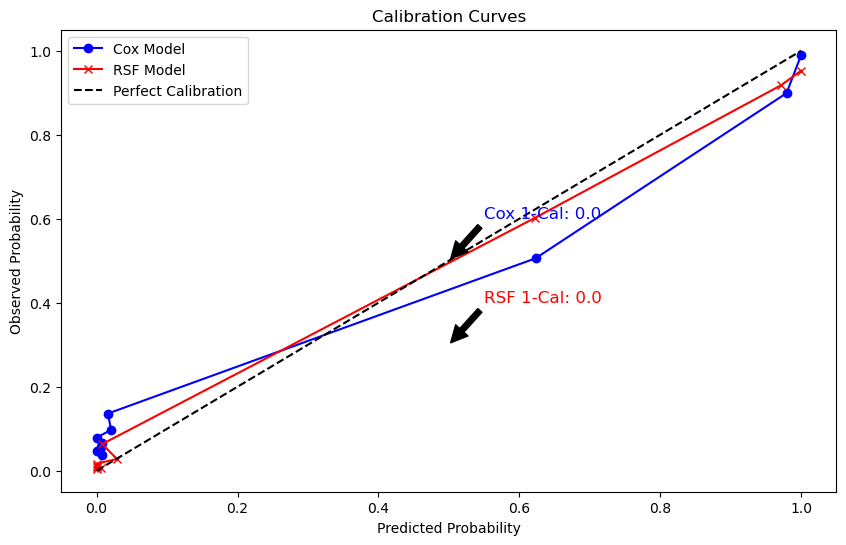
\includegraphics[scale=0.6]{Figures/SURV/calibration.png}
    \caption{One Calibration Errors}
    \label{fig:your_label}
\end{figure}

\begin{figure}[h]
    \centering
    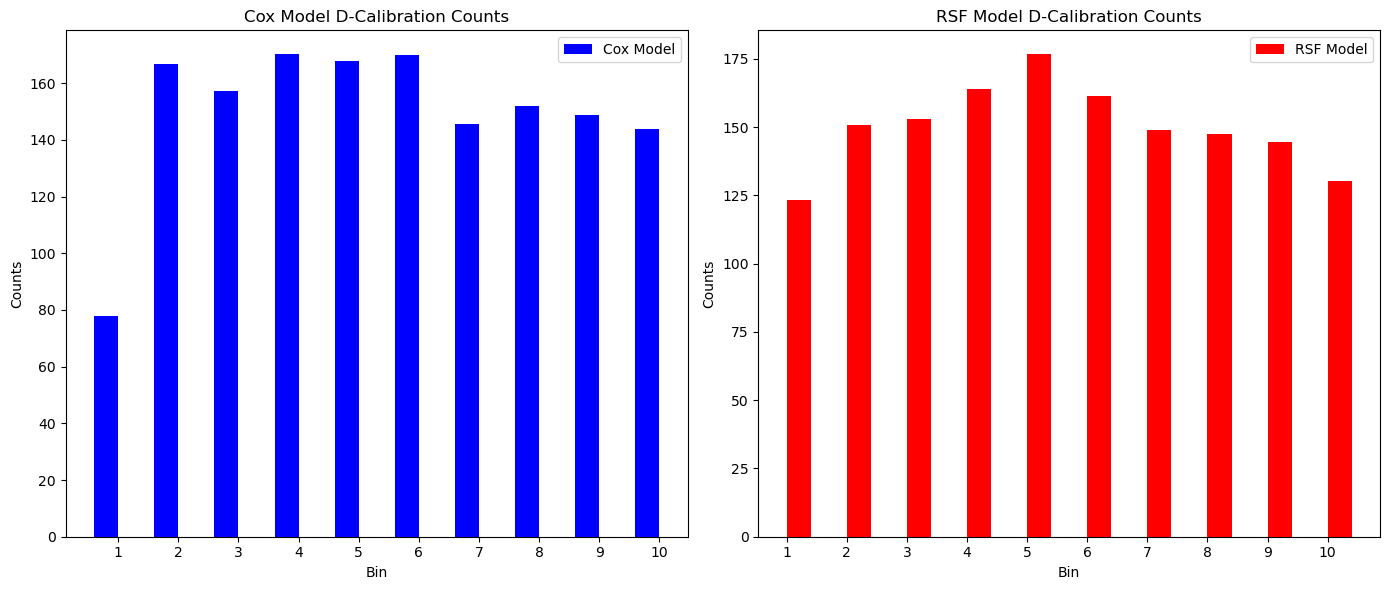
\includegraphics[width=\linewidth]{Figures/SURV/binned_d_cal.png}
    \caption{Binned D-calibration Errors}
    \label{fig:your_label}
\end{figure}


